\documentclass[12pt]{article}\usepackage[]{graphicx}\usepackage[]{xcolor}
% maxwidth is the original width if it is less than linewidth
% otherwise use linewidth (to make sure the graphics do not exceed the margin)
\makeatletter
\def\maxwidth{ %
  \ifdim\Gin@nat@width>\linewidth
    \linewidth
  \else
    \Gin@nat@width
  \fi
}
\makeatother

\definecolor{fgcolor}{rgb}{0.345, 0.345, 0.345}
\newcommand{\hlnum}[1]{\textcolor[rgb]{0.686,0.059,0.569}{#1}}%
\newcommand{\hlstr}[1]{\textcolor[rgb]{0.192,0.494,0.8}{#1}}%
\newcommand{\hlcom}[1]{\textcolor[rgb]{0.678,0.584,0.686}{\textit{#1}}}%
\newcommand{\hlopt}[1]{\textcolor[rgb]{0,0,0}{#1}}%
\newcommand{\hlstd}[1]{\textcolor[rgb]{0.345,0.345,0.345}{#1}}%
\newcommand{\hlkwa}[1]{\textcolor[rgb]{0.161,0.373,0.58}{\textbf{#1}}}%
\newcommand{\hlkwb}[1]{\textcolor[rgb]{0.69,0.353,0.396}{#1}}%
\newcommand{\hlkwc}[1]{\textcolor[rgb]{0.333,0.667,0.333}{#1}}%
\newcommand{\hlkwd}[1]{\textcolor[rgb]{0.737,0.353,0.396}{\textbf{#1}}}%
\let\hlipl\hlkwb

\usepackage{framed}
\makeatletter
\newenvironment{kframe}{%
 \def\at@end@of@kframe{}%
 \ifinner\ifhmode%
  \def\at@end@of@kframe{\end{minipage}}%
  \begin{minipage}{\columnwidth}%
 \fi\fi%
 \def\FrameCommand##1{\hskip\@totalleftmargin \hskip-\fboxsep
 \colorbox{shadecolor}{##1}\hskip-\fboxsep
     % There is no \\@totalrightmargin, so:
     \hskip-\linewidth \hskip-\@totalleftmargin \hskip\columnwidth}%
 \MakeFramed {\advance\hsize-\width
   \@totalleftmargin\z@ \linewidth\hsize
   \@setminipage}}%
 {\par\unskip\endMakeFramed%
 \at@end@of@kframe}
\makeatother

\definecolor{shadecolor}{rgb}{.97, .97, .97}
\definecolor{messagecolor}{rgb}{0, 0, 0}
\definecolor{warningcolor}{rgb}{1, 0, 1}
\definecolor{errorcolor}{rgb}{1, 0, 0}
\newenvironment{knitrout}{}{} % an empty environment to be redefined in TeX

\usepackage{alltt}
\usepackage{amsmath}
\usepackage{graphicx}
%\usepackage{enumerate}
\usepackage{natbib}
\usepackage{url} % not crucial - just used below for the URL

\usepackage[utf8]{inputenc} % allow utf-8 input
% \usepackage[T1]{fontenc}    % use 8-bit T1 fonts
\usepackage{hyperref}       % hyperlinks
\usepackage{url}            % simple URL typesetting
\usepackage{booktabs}       % professional-quality tables
\usepackage{amsfonts}       % blackboard math symbols
\usepackage{nicefrac}       % compact symbols for 1/2, etc.
\usepackage{microtype}      % microtypography
\usepackage{graphicx}
\usepackage{natbib}
\usepackage{doi}

% extra packages
\usepackage{longtable}
\usepackage{colortbl}
\usepackage{amsmath}
\usepackage{caption}
\usepackage{multirow}
\hypersetup{hidelinks}
\usepackage{geometry}
\usepackage{pdflscape}
\usepackage{bm}
\usepackage{algorithm, algcompatible, algpseudocode}
\usepackage{eqparbox}

\DeclareMathOperator*{\argmin}{argmin}
\DeclareMathOperator*{\argmax}{argmax}

\newdimen{\algindent}
\setlength\algindent{1.5em}          % algorithmic indent=1.5em
\algnewcommand\LeftComment[2]{%
\hspace{#1\algindent}$\triangleright$ \eqparbox{COMMENT}{#2} \hfill %
}

\algnewcommand{\algorithmicgoto}{\textbf{go to}}%
\algnewcommand{\Goto}[1]{\algorithmicgoto~\ref{#1}}%

\DeclareCaptionLabelFormat{AppendixTables}{A.#2}

\definecolor{lightgray}{rgb}{0.83, 0.83, 0.83}

% Definitions of handy macros can go here

\newcommand{\dataset}{{\cal D}}
\newcommand{\fracpartial}[2]{\frac{\partial #1}{\partial  #2}}
\newcommand{\ie}{\textit{i.e.}}
\newcommand{\eg}{\textit{e.g.}}
\newcommand{\cstat}{\widehat{\text{C}}(t)}
\newcommand{\bstat}{\widehat{\text{BS}}(t)}
\newcommand{\bsbar}{\mathcal{\widehat{BS}}(t_1, t_2)}
\newcommand{\bskap}{\mathcal{\widehat{BS}}_0(t_1, t_2)}

\newcommand{\ntrain}{N_{\text{train}}}
\newcommand{\ntest}{N_{\text{test}}}

\newcommand{\secref}[1]{Section \ref{#1}}

\newcommand{\tabref}[1]{Table \ref{#1}}
\newcommand{\tabrefAppendix}[1]{Table A.\ref{#1}}

\newcommand{\nope}[1]{}


%\pdfminorversion=4
% NOTE: To produce blinded version, replace "0" with "1" below.
\newcommand{\blind}{1}

% DON'T change margins - should be 1 inch all around.
\addtolength{\oddsidemargin}{-.5in}%
\addtolength{\evensidemargin}{-.5in}%
\addtolength{\textwidth}{1in}%
\addtolength{\textheight}{1.3in}%
\addtolength{\topmargin}{-.8in}%



\IfFileExists{upquote.sty}{\usepackage{upquote}}{}
\begin{document}

%\bibliographystyle{natbib}

\def\spacingset#1{\renewcommand{\baselinestretch}%
{#1}\small\normalsize} \spacingset{1}


%%%%%%%%%%%%%%%%%%%%%%%%%%%%%%%%%%%%%%%%%%%%%%%%%%%%%%%%%%%%%%%%%%%%%%%%%%%%%%

\if0\blind
{
  \title{\bf Accelerated and interpretable oblique random survival forests}
  \author{Byron C.~Jaeger\thanks{
    The authors gratefully acknowledge \textit{the Center for Biomedical Informatics, Wake Forest University School of Medicine for supporting this research. The project was also supported by the National Center for Advancing Translational Sciences (NCATS), National Institutes of Health through Grant Award Number UL1TR001420. The content is solely the responsibility of the authors and does not necessarily represent the official views of the NIH. Dr. Pajewski was supported by grant number P30AG021332 from the National Institutes of Health, while Dr. Speiser was supported by K25AG068253.}}\hspace{.2cm}\\
   Dept. of Biostatistics and Data Science,
	 Wake Forest Univ. School of Medicine\\
  and \\
   Sawyer Welden \\
   Dept. of Biostatistics and Data Science,
   Wake Forest Univ. School of Medicine \\
  and \\
   Kristin Lenoir \\
   Dept. of Biostatistics and Data Science,
   Wake Forest Univ. School of Medicine\\
  and \\
   Jaime L.~Speiser \\
	 Dept. of Biostatistics and Data Science,
	 Wake Forest Univ. School of Medicine\\
	and \\
	 Matthew W. Segar \\
   Dept. of Cardiology,
   Texas Heart Institute \\
  and \\
   Ambarish Pandey \\
   Division of Cardiology, Dept. of Internal Medicine, \\
   University of Texas Southwestern Medical Center \\
  and \\
   Nicholas M.~Pajewski \\
	 Dept. of Biostatistics and Data Science,
	 Wake Forest Univ. School of Medicine
  }
  \maketitle
} \fi

\if1\blind
{
  \bigskip
  \bigskip
  \bigskip
  \begin{center}
    {\LARGE\bf Accelerated and interpretable oblique random survival forests}
\end{center}
  \medskip
} \fi

\newpage
\begin{abstract}
	The oblique random survival forest (RSF) is an ensemble supervised learning method for right-censored outcomes. Trees in the oblique RSF are grown using linear combinations of predictors, whereas in the standard RSF, a single predictor is used. Oblique RSF ensembles have high prediction accuracy, but assessing many linear combinations of predictors induces high computational overhead. In addition, few methods have been developed for estimation of variable importance (VI) with oblique RSFs. We introduce a method to increase computational efficiency of the oblique RSF and a method to estimate VI with the oblique RSF. Our computational approach uses Newton-Raphson scoring in each non-leaf node, We estimate VI by negating each coefficient used for a given predictor in linear combinations, and then computing the reduction in out-of-bag accuracy. In benchmarking experiments, we find our implementation of the oblique RSF is hundreds of times faster, with equivalent prediction accuracy, compared to existing software for oblique RSFs. We find in simulation studies that `negation VI' discriminates between relevant and irrelevant numeric predictors more accurately than permutation VI, Shapley VI, and a technique to measure VI using analysis of variance. All  oblique RSF methods in the current study are available in the \texttt{aorsf} R package, and additional supplemental materials are available online.
\end{abstract}

\noindent%
{\it Keywords:}  Supervised learning, Computational efficiency, Variable importance
\vfill

\newpage
\spacingset{1.5} % DON'T change the spacing!

\section{Introduction}

Risk prediction may reduce the burden of disease by guiding strategies for prevention and treatment in a wide range of domains \citep{moons2012riskI}. The random survival forest (RSF; \citet{ishwaran2008random, hothorn2006unbiased}) is a supervised learning algorithm that has been used frequently for risk prediction \citep{wang2017selective}. Similar to random forests (RFs) for classification and regression \citep{breiman2001random}, The RSF is a large set of de-correlated and randomized decision trees, with each tree contributing to the ensemble's prediction function. Notable characteristics of the RSF include uniform convergence of its ensemble survival prediction function to the true survival function, first shown by \citet{ishwaran2010consistency} and later by \citet{cui2017consistency} under more general conditions. However, \citet{cui2017consistency} noted that the RSF is at a disadvantage when predictors are correlated and some are not relevant to the censored outcome, which is a strong possibility when large clinical and `omic' databases are leveraged for risk prediction.

A potential approach to improve the RSF when predictors are correlated and some are not relevant to the censored outcome is to use oblique trees instead of axis based trees. Axis based trees split data using a single predictor, creating decision boundaries that are perpendicular or parallel to axes of the predictor space \citep[see][Chapter~2]{breiman2017classification}. Oblique trees split data using a linear combination of predictors, creating decision boundaries that are neither parallel nor perpendicular to axes of their contributing predictors \citep[see][Chapter~5]{breiman2017classification}. Oblique trees may create more adequate partitions of a predictor space compared to axis-based trees, as demonstrated in Figure \ref{fig:axis_v_oblique}. \citet{menze2011oblique} examined prediction accuracy of RFs in the presence of correlated predictors and found that oblique RFs had substantially higher prediction accuracy compared to axis-based RFs. Similarly, \citet{jaeger2019oblique} found that growing RSFs with oblique rather than axis-based trees reduced the RSF's concordance error, with improvements ranging from 2.5\% to 24.9\% depending on the data analyzed.

\begin{knitrout}
\definecolor{shadecolor}{rgb}{0.969, 0.969, 0.969}\color{fgcolor}\begin{figure}
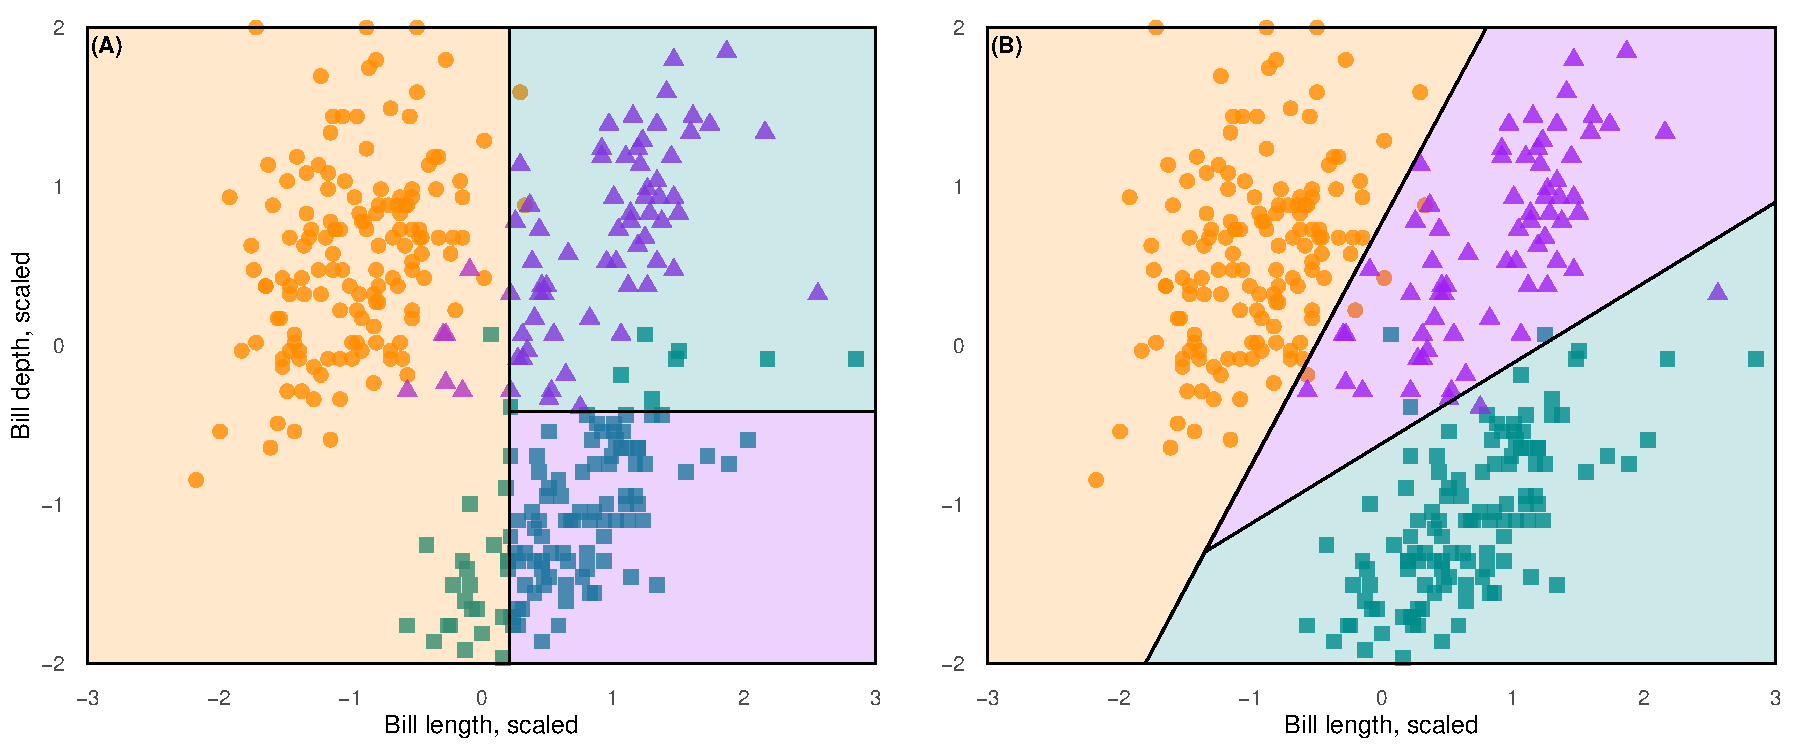
\includegraphics[width=\maxwidth]{figure/axis_v_oblique-1} \caption[Decision boundaries from an axis based (panel A) and oblique (panel B) decision tree used to classify penguin species based on bill depth and bill length]{Decision boundaries from an axis based (panel A) and oblique (panel B) decision tree used to classify penguin species based on bill depth and bill length. The decision boundary from the oblique tree is better able to capture the geometry of this data, leading to fewer mis-classified penguins.}\label{fig:axis_v_oblique}
\end{figure}

\end{knitrout}


Conceptually, oblique trees are similar to methods that use covariate rotation or extension to generate linear combinations of predictors prior to growing axis-based trees \citep{zhou2016random, wang2017random}. The difference is that oblique trees generate linear combinations of predictors within each non-leaf node, using only the data and predictors associated with that node, instead of generating the linear combinations prior to growing the tree. This ``node-specific'' approach to creating linear combinations of predictors leads to greater diversity in oblique tree ensembles, which may lead to greater prediction accuracy \citep{breiman2001random}.

Despite the potential for higher accuracy, oblique trees have at least two notable drawbacks compared to axis-based trees. First, finding a locally optimal oblique decision rule may require exponentially more computation than an axis-based rule. If $p$ predictors are potentially used to split $n$ observations, up to $\mathcal{O}(n^p)$ oblique splits can be assessed versus $\mathcal{O}(n \cdot p)$ axis-based splits \citep{heath1993induction, murthy1994system}. Second, although variable importance (VI) is one of the most widely used strategies to interpret RFs \citep{ishwaran2019standard}, few studies have investigated VI for oblique RFs \citep[see][Section~5]{menze2011oblique}, and fewer have investigated VI specifically for the oblique RSF. Without general methodology to estimate VI, interpretation of oblique RFs is challenging.

The aim of this paper is to introduce methodology that improves the computational efficiency and interpretation of oblique RSFs. \secref{sec:methods} reviews prior work, introduces our method to reduce the computational cost of oblique RSFs (\ie, accelerate them), and introduces `negation VI', a method to estimate VI with oblique RSFs that does not require permutation of data. We describe benchmarking experiments and simulation studies to evaluate these methods in \secref{sec:numeric}, and present results in \secref{sec:results}. In \secref{sec:discussion}, we summarize results from the current study, connecting our findings to prior work and outlining potential future research topics. All oblique RSF methods introduced in the current study are available in the \texttt{aorsf} R package \citep{jaeger2022aorsf}.

\section{Methods and materials} \label{sec:methods}

Sections \ref{sec:rw_forests} and \ref{sec:rw_vi} briefly summarize prior studies that have developed methods related to the oblique RSF and VI, respectively. \secref{sec:aorsf} describes our approach to reduce computational overhead of the oblique RSF and \secref{sec:negation_vi} introduces negation VI, a novel technique to estimate VI in oblique RFs.

\subsection{Axis-based and oblique random forests} \label{sec:rw_forests}

After \citet{breiman2001random} introduced the axis-based and oblique RF, numerous methods were developed to grow oblique RFs for classification or regression tasks \citep{menze2011oblique, zhang2014oblique, rainforth2015canonical, zhu2015reinforcement, poona2016investigating, qiu2017oblique, tomita2020sparse, katuwal2020heterogeneous}. However, oblique splitting approaches for classification or regression may not generalize to censored outcomes \citep[\eg, see][Section~4.5.1]{zhu2013tree}, and most research involving the RSF has focused on forests with axis-based trees \citep{wang2017selective}.

\citet{hothorn2006unbiased} developed an axis-based RSF in their framework for unbiased recursive partitioning, more commonly referred to as the conditional inference forest (CIF). \citet{zhou2016random} developed a rotation forest based on the CIF and \citet{wang2017random} developed a method for extending the predictor space of the CIF. \citet{ishwaran2008random} developed an axis-based RSF with strict adherence to the rules for growing trees proposed in \citet{breiman2001random}.  \citet{jaeger2019oblique} developed the oblique RSF following the bootstrapping approach described in Breiman's original RF and incorporating early stopping rules from the CIF.

Fast algorithms to fit axis-based RSFs are available in the \texttt{randomForestSRC} R package \citep{randomForestSRC} and the \texttt{ranger} \citep{ranger} R package. \texttt{randomForestSRC} provides a unified interface to grow RFs in a wide range of analyses, and \texttt{ranger} is designed to grow RFs efficiently using high dimensional data. Fast algorithms to fit the CIF are provided by the \texttt{party} R package \citep{hothorn2010party}, which provides a computational toolbox for recursive partitioning using conditional inference trees. \citet{jaeger2019oblique} developed the \texttt{obliqueRSF} package and found it was approximately 30 times slower than \texttt{party} and nearly 200 times slower than \texttt{randomForestSRC}. Few studies have developed software with fast algorithms for oblique RSFs that have comparable speed compared to algorithms for axis-based RSFs.

\subsection{Variable importance} \label{sec:rw_vi}

Several techniques to estimate VI have been developed since \citet{breiman2001random} introduced permutation VI, which is defined for each predictor as the difference in a RF's estimated prediction error before versus after the predictor's values are randomly permuted. \citet{strobl2007bias} identified bias in permutation VI driven by categorical predictors and bootstrap sampling, and proposed a permutation VI measure based on unbiased recursive partitioning \citep{hothorn2006unbiased}. \citet{menze2011oblique} introduced an approach to estimate VI for oblique RFs that computes an analysis of variance (ANOVA) table in non-leaf nodes to obtain p-values for each predictor contributing to the node. The ANOVA VI\footnote{\citet{menze2011oblique} name their method `oblique RF VI', but we use the name `ANOVA VI' in this article to avoid confusing Menze's approach with other approaches to estimate VI for oblique RFs.} is then defined for each predictor as the number of times a p-value associated with the predictor is $\leq 0.01$ while growing a forest. \citet{lundberg2017unified} introduced a method to estimate VI using SHapley Additive exPlanation (SHAP) values, which estimates the contribution of a predictor to a model's prediction for a given observation. SHAP VI is computed for each predictor by taking the mean absolute value of SHAP values for that predictor across all observations in a given set. With the exception of \citet{menze2011oblique}, few studies have evaluated estimation of VI using oblique RFs, and fewer have examined VI specifically for the oblique RSF.

% Several supervised learning algorithms can develop prediction functions for right-censored time-to-event outcomes, henceforth referred to as survival outcomes. \cite{ishwaran2008random} developed the RF for survival, an extension of the RF for regression and classification developed by \citet{breiman2001random}.

\subsection{The accelerated oblique random survival forest} \label{sec:aorsf}

Consider the usual framework for right-censored time-to-event outcomes with training data $$\dataset_{\text{train}} = \left\{ (T_i, \delta_i, \bm{x}_{i}) \right\}_{i=1}^{N_{\text{train}}}.$$ Here, $T_i$ is the event time if $\delta_i=1$ or the censoring time if $\delta_i=0$, and $\bm{x}_i$ is a vector of predictors values. Assuming there are no ties, let $t_1 < \, \ldots \, < t_m$ denote the $m$ unique event times in $\dataset_{\text{train}}$.

To accelerate the oblique RSF, we propose to identify linear combinations of predictor variables in non-leaf nodes by applying Newton Raphson scoring to the partial likelihood function of the Cox regression model:
\begin{equation}\label{eqn:cox-partial-likelihood}
L(\bm\beta) = \prod_{i=1}^m \frac{e^{\bm{x}_{j(i)}^T \bm\beta}}{\sum_{j \in R_i} e^{\bm{x}_j^T \bm\beta}},
\end{equation}
where $R_i$ is the set of indices, $j$, with $T_j \geq t_i$ (\ie, those still at risk at time $t_i$), and $j(i)$ is the index of the observation for which an event occurred at time $t_i$. Newton Raphson scoring is an exceptionally fast estimation procedure, and the \texttt{survival} package \citep{survival} includes documentation that outlines how to efficiently program it \citep{therneau_survival_2022}. As described in \cite{therneau2000cox}, a vector of estimated regression coefficients, $\hat{\bm{\beta}}$, is updated in each step of the procedure: $$\hat{\bm{\beta}}^{k+1} =  \hat{\bm{\beta}}^{k} + U(\hat{\bm{\beta}} = \hat{\bm{\beta}}^{k})\, \mathcal{I}^{-1}(\hat{\bm{\beta}} = \hat{\bm{\beta}}^{k}),$$ where $U(\hat{\bm{\beta}})$ is the score vector and $\mathcal{I}^{-1}(\hat{\bm{\beta}})$ is the inverse of the observed information matrix. After obtaining $\hat{\bm\beta}$, a linear combination of variables, $\eta$, is obtained by computing $\eta = \bm{x}^T \hat{\bm{\beta}}$.


For statistical inference, it is recommended to continue updating $\hat{\bm{\beta}}$ by completing additional iterations of Newton Raphson scoring until a convergence threshold is met. However, since an estimate of $\hat{\bm{\beta}}$ is created by the first iteration of Newton Raphson scoring, only one iteration of Newton Raphson scoring is needed to identify a valid linear combination of predictors. In \secref{sec:results_pred}, we formally test whether growing oblique survival trees using one iteration of Newton Raphson scoring provides equivalent prediction accuracy compared to trees where iterations are completed until a convergence threshold is met.

Algorithm \ref{alg:aorsf} presents our approach to fitting an oblique survival tree in the accelerated oblique RSF using default values from the \texttt{aorsf} R package. Several steps are taken to reduce computational overhead. First, memory is conserved by conducting bootstrap resampling via random integer-valued weights, rather than using a bootstrapped copy of the original data. Memory conservation also takes place in terminal nodes, where we restrict estimation of the survival and cumulative hazard function to event times that occur among observations in the node. Second, early stopping is applied to the tree-growing procedure if a statistical criterion is not met. In our case, the criterion is based on the magnitude of a log-rank test statistic corresponding to splitting the data at a current node. Third, instead of greedy recursive partitioning, we use `good enough' partitioning. More specifically, instead of computing a log-rank test statistic for several different linear combinations of variables and proceeding with the highest scoring option, we identify an optimal cut-point for one linear combination of variables and assess whether using this combination will create a split that passes the criterion for splitting a node. If it does not pass the criterion, then another linear combination will be tested, with the maximum number of attempts set by the parameter \texttt{n\_retry}. Often a `good-enough` split can be found in just one attempt when the training set is large, which gives the accelerated oblique RSF a computational advantage in larger training sets compared to greedy partitioning.

\spacingset{1}
\begin{algorithm}
    \caption{Accelerated oblique random survival tree using default parameters.} \label{alg:aorsf}
  \begin{algorithmic}[1]
    \Require Training data $\dataset_{\text{train}} = \left\{ (T_i, \delta_i, \bm{x}_{i}) \right\}_{i=1}^{N_{\text{train}}}$, $\text{mtry} = \sqrt{\text{ncol}(\bm{x}_{\text{train}})}$, $\text{n\_split} = 5$, $\text{n\_retry} = 3$, and $\text{split\_min\_stat} = 3.841459$
    \State $\mathcal{T} \gets \emptyset$
    \State $w \gets \text{sample}(\text{from} = \left\{0, \ldots, 10\right\},\,\text{size} = \text{nrow}(\bm{x}_{\text{train}}),\, \text{replace} = \text{T})$
    \State $\dataset_{\text{in-bag}} \gets \text{subset}(\dataset_{\text{train}},\,\text{rows} = \text{which}(w > 0))$
    \State $w \gets \text{subset}(w,\, \text{which}(w > 0))$
    \State $\text{node\_assignments} \gets \text{rep}(1,\,\text{times} = \text{nrow}(\bm{x}_{\text{in-bag}}))$
    \State $\text{nodes\_to\_split} \gets \{1\}$
     \While {$\text{nodes\_to\_split} \neq \emptyset$}
     \For{$\text{node} \in \text{nodes\_to\_split}$}
       \State $\text{n\_try} \gets 1$
       \State $\text{node\_rows} \gets \text{which}(\text{node\_assignments} \equiv \text{node})$
       \State $\text{node\_cols} \gets \text{sample}(\text{from} = \left\{1, \ldots, \text{ncol}(\bm{x})\right\},\, \text{size} = \text{mtry},\,\text{replace} = \text{F})$ \label{marker}
       \State $\dataset_{\text{node}} \gets \text{subset}(\dataset_{\text{in-bag}},\,\text{rows} = \text{node\_rows},\,\text{columns} = \text{node\_cols})$
       \State $\beta \gets \text{newt\_raph}(\dataset_{\text{node}},\, \text{weights} = \text{subset}(w, \text{node\_rows}),\, \text{max\_iter} = 1)$
       \State $\eta \gets \bm{x}^T_{\text{node}} \times \beta$
       \State $\mathcal{C} \gets \text{sample}(\text{from} = \text{unique}(\eta),\, \text{size} = \text{n\_split},\,\text{replace} = \text{F})$
       \State $c \gets \argmax_{c^* \in \mathcal{C}} \left\{ \text{log\_rank\_stat}(\eta, c^*) \right\}$
       \If{$\text{log\_rank\_stat}(\eta, c) \geq \text{split\_min\_stat}$}
         \State $\mathcal{T} \gets \text{add\_node}(\mathcal{T},\, \text{name} = \text{node},\, \text{beta} = \beta,\, \text{cutpoint} = c)$
         \State \LeftComment{0}{Right node logic omitted for brevity (identical to left node logic)}
         \State $\text{node\_left\_name} \gets \text{max}(\text{node\_assignments}) + 1$
         \State $\text{node\_left\_rows} \gets \text{subset}(\text{node\_rows},\,\text{which}(\eta \leq c))$
         \State $\text{subset}(\text{node\_assignments}, \text{node\_left\_rows}) \gets \text{node\_left\_name}$
         \If{$\text{is\_splittable}(\text{subset}(\text{node\_assignments}, \text{node\_left\_rows}))$}
           \State $\text{nodes\_to\_split} \gets \text{nodes\_to\_split} \cup \text{node\_left\_name}$
         \Else
           \State $\mathcal{T} \gets \text{add\_leaf}(\mathcal{T},\, \text{data} = \text{subset}(\dataset_{\text{node}},\,\text{rows} = \text{node\_left\_rows}))$
         \EndIf
       \ElsIf{$\text{n\_try} \leq \text{n\_retry}$}
         \State $\text{n\_try} \gets \text{n\_try} + 1$
         \State \Goto{marker}
       \Else
         \State $\mathcal{T} \gets \text{add\_leaf}(\mathcal{T},\, \text{data} =\dataset_{\text{node}})$
       \EndIf
       \State $\text{nodes\_to\_split} \gets \text{nodes\_to\_split} \setminus \{\text{node}\}$
     \EndFor
  \EndWhile
  \State \Return $\mathcal{T}$
  \end{algorithmic}
\end{algorithm}
\spacingset{1.5}

\subsection{Negation variable importance} \label{sec:negation_vi}

This Section introduces negation VI, which is similar to permutation VI in that it measures how much a model’s prediction error increases when a variable’s role in the model is de-stabilized. Specifically, negation VI measures the increase in an oblique RF's prediction error after flipping the sign of all coefficients linked to a variable (\ie, negating them). As negating a coefficient effectively flips decision boundaries around the corresponding predictor's axis, scaling numeric predictors to have a mean of zero and standard deviation of one is recommended.\footnote{The \texttt{aorsf} package automatically scales numeric inputs to a mean of zero and standard deviation of one.} For the current study, we use Harrell's concordance (C)-statistic \citep{harrell1982evaluating} to measure change in prediction error when computing negation VI.

% A motivating problem for negation VI is that of correlated, numeric predictors. When two predictors are correlated and only one of them is relevant for prediction of an outcome, VI methods based on permutation are known to have upward bias in estimating the importance of the irrelevant predictor \citep{hooker2021unrestricted}. Permutation may distort the joint distribution of predictors, which may in turn increase a model's estimated prediction error due to extrapolation. On the other hand, negating coefficients modifies the decision rule rather than modifying the data. Thus, we hypothesize that negation VI can be more effective at identifying important predictors for correlated, numeric predictors.

To demonstrate negation VI, consider a classification task where the goal is prediction of penguin species (chinstrap, gentoo, or adelie) based on bill length and bill depth \citep{palmerpenguins_rpack}. Scaling these predictors to be centered at 0, we find oblique decision boundaries defined by linear combinations of bill length and bill depth correctly classify most of the data (Figure \ref{fig:negation}, Panel A). Permuting the values of bill length leads to several mis-classified observations, suggesting that bill length is an important predictor (Figure \ref{fig:negation}, Panel B). However, inspecting the permuted data shows that a number of observations moved to a region in the predictor space where there were previously no observations. Moving data to unobserved or perhaps unobservable regions of the predictor space may cause extrapolation error, which \citet{hooker2021unrestricted} identified as a cause of bias in permutation importance. Negating the coefficients for bill length in the linear combinations that define our decision boundaries causes the boundaries to flip across bill length's axis (Figure \ref{fig:negation}, Panel C). This leads to several mis-classified observations, suggesting that bill length is an important predictor without distorting the joint distribution of bill length and bill depth.

Negation VI is an extension of ``anti VI", a VI technique for axis-based trees which became the default VI method for \texttt{randomForestSRC} in version 2.14.0. Anti VI reverses the direction of all decision nodes that use a specific variable, and then reassesses the ensemble prediction error. So, if an axis-based decision rule were defined as $x > 5 \Rightarrow$ send data to right node, the decision rule would become $x > 5 \Rightarrow$ send data to left node when computing the importance of a predictor $x$. Put in a way that makes the connection to negation VI more explicit, the `noised up' decision rule can be written as $-x > 5 \Rightarrow$ send data to right node.

\begin{knitrout}
\definecolor{shadecolor}{rgb}{0.969, 0.969, 0.969}\color{fgcolor}\begin{figure}
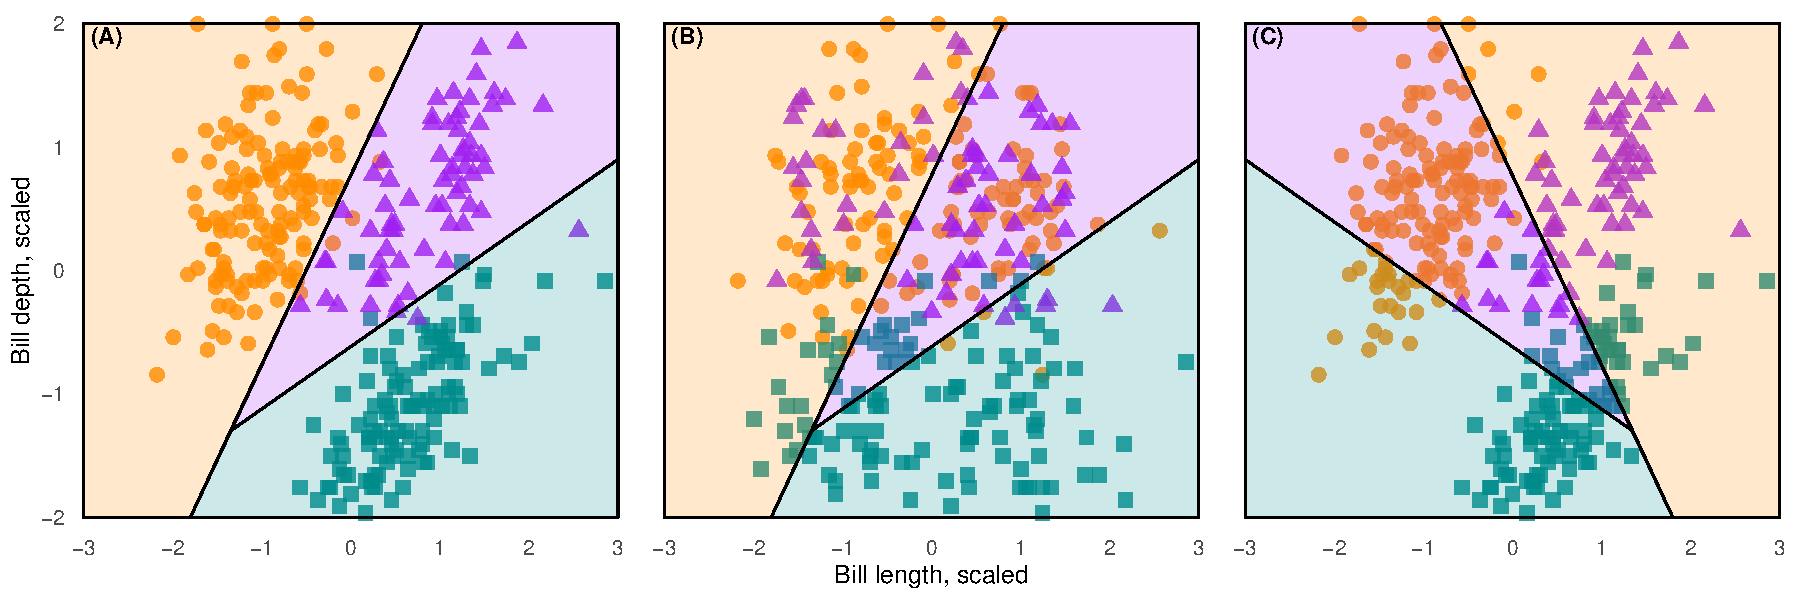
\includegraphics[width=\maxwidth]{figure/negation-1} \caption[Demonstration of negation and permutation importance for a single oblique tree]{Demonstration of negation and permutation importance for a single oblique tree. Panel A shows the original data and decision boundaries. Panel B shows the data with permuted bill length values. Panel C shows the decision boundaries after negating coefficients for bill length. Permutation and negation both show that bill length is an important predictor, but permuting bill length distorts its joint distribution with bill depth.}\label{fig:negation}
\end{figure}

\end{knitrout}


Negation VI has several strengths. First, it generalizes to any oblique RF (\ie, not just RSFs) using any valid error function, making it both general and flexible.\footnote{The \texttt{aorsf} package enables customized functions to be applied in lieu of the default C-statistic.} Second, negation is non-random, making it reproducible without setting a random seed and making it slightly faster than permutation importance. Fourth, since negation VI does not permute variables, the analyst need not worry about impossible combinations of predictors that may occur when one predictor is randomly permuted, such as having a negative status for type 2 diabetes and having Hemoglobin A1c level $\geq$ 6.5\% (a value indicative of type 2 diabetes) as a result of randomly permuting the values of Hemoglobin A1c. However, in scenarios where decision boundaries have symmetry around the origin of the predictor space (\eg, all positive cases lie in a circle centered at the origin, with negative cases sitting outside the circle), negation importance will be less effective than permutation.


\section{Numeric experiments} \label{sec:numeric}



Sections \ref{sec:bm_pred} and \ref{sec:bm_vi} present the design of numerical experiments examining the accelerated oblique RSF and negation VI, respectively. \secref{sec:bm_compute} summarizes our approach to evaluating computational efficiency of learning algorithms, with a focus on the accelerated oblique RSF and other RSF implementations. \secref{sec:computing} provides details on computation and code.

\subsection{Benchmark of prediction accuracy} \label{sec:bm_pred}

The aim of this numeric experiment is to evaluate the prediction accuracy of the accelerated oblique RSF compared to its predecessor (the oblique RSF from the \texttt{obliqueRSF} R package) and to several other machine learning algorithms. Inferences drawn from this experiment include equivalence and inferiority tests based on Bayesian linear mixed models.

\subsubsection{Learners} \label{sec:learners}

We consider four classes of learners: RSFs (both axis-based and oblique), boosting ensembles, regression models, and neural networks. Specific learners from each class are summarized in \tabref{tab:learners}. To facilitate fair comparisons, tuning parameters were harmonized within each class. For example, for RSF learners, we set the minimum node size (a parameter shared by all RSF learners) as 10. Additionally, for RSF learners, the number of randomly selected predictors was the square root of the total number of predictors rounded to the nearest integer, and the number of trees in the ensemble was 500 (a common default value for the number of trees). For boosting, regression, and neural network learners, nested cross-validation was applied to tune relevant model parameters. Nested cross-validation includes an `inner' cross-validation loop to evaluate different specifications of tuning parameters and an `outer' loop that evaluates the tuned model, providing an unbiased estimate of the underlying model and its tuning procedure. Tuning for boosting models included identifying the number of steps to complete. The maximum number of steps was 5000, the learning rate was fixed at 0.01, and early stopping was applied if there was no improvement in cross-validated negative log-likelihood for 25 steps. For regression models, tuning was used to identify the magnitude of penalization. For neural networks, the number of layers (\ie, length) and number of nodes in the layers (\ie, width) was tuned, while dropout rate was fixed at 10\%, batch size was fixed at 32 observations, and the rectified linear unit activation function was applied. In addition, neural networks completed a maximum of 500 epochs, with possible early stopping based on prediction accuracy in a validation set comprising 25\% of its training data..

\newgeometry{margin=1cm} % modify this if you need even more space
\begin{landscape}
\spacingset{1}
\begin{table}[h!]
\centering
\begin{tabular}{p{2cm} | p{3cm} p{4cm} p{12cm}}
 \hline
 Learner Class & Software & Learners & Description \\ [0.5ex]
 \hline\hline
 \multicolumn{3}{l}{\textit{Random Survival Forests}}\\
 \hline\hline

 Axis based &

 \href{https://www.randomforestsrc.org/index.html}{\texttt{RandomForestSRC}} \newline
 \href{https://CRAN.R-project.org/package=ranger}{\texttt{ranger}} \newline
 \href{http://party.r-forge.r-project.org/}{\texttt{party}} \newline
 \href{https://github.com/whcsu/rotsf}{\texttt{rotsf}} \newline
 \href{https://github.com/whcsu/rsfse}{\texttt{rsfse}} &

 \texttt{rsf-standard} \newline
 \texttt{rsf-extratrees} \newline
 \texttt{cif-standard} \newline
 \texttt{cif-rotate} \newline
 \texttt{cif-spacextend} &

 \texttt{rsf-standard} grows survival trees following Leo Breiman's random forest algorithm with cut-points selected to maximize a log-rank statistic. \texttt{rsf-extratrees} grows survival trees with randomly selected predictors and cut-points. \texttt{cif-standard} uses conditional inference. \texttt{cif-rotate} extends \texttt{cif-standard} by applying principal component analysis to random subsets of data prior to growing each survival tree. \texttt{cif-spacextend} derives new predictors for each tree in the ensemble, separately. \\ \hline


 Oblique &


 \href{https://CRAN.R-project.org/package=obliqueRSF}{\texttt{obliqueRSF}} \newline
 \href{https://bcjaeger.github.io/aorsf/}{\texttt{aorsf}} &

 \texttt{obliqueRSF-net} \newline
 % \texttt{aorsf-net} \newline
 \textcolor{purple}{\texttt{aorsf-fast}} \newline
 \texttt{aorsf-cph} \newline
 \texttt{aorsf-extratrees} &


 Oblique survival trees following Leo Breiman's random forest algorithm. Linear combinations of inputs are derived using \texttt{glmnet} in \texttt{obliqueRSF-net}, using Newton Raphson scoring for the Cox partial likelihood function in \texttt{aorsf-fast} (1 iteration of scoring) and \texttt{aorsf-cph} (up to 20 iterations), and chosen randomly from a uniform distribution in \texttt{aorsf-extratrees}. Cut-points are selected to maximize a log-rank statistic. \\

 \hline\hline
 \multicolumn{3}{l}{\textit{Boosting ensembles}}\\
 \hline\hline

 Trees &

 \href{https://xgboost.readthedocs.io/en/stable/#}{\texttt{xgboost}} &

 \texttt{xgboost-cox} \newline
 \texttt{xgboost-aft} &

 \texttt{xgboost-cox} maximizes the Cox partial likelihood function, whereas \texttt{xgboost-aft} maximizes the accelerated failure time likelihood function. Nested cross validation (5 folds) is applied to tune the number of trees. The minimum number of observations in a leaf node was 10, the maximum depth of trees was 6, and $\sqrt{p}$ variables were considered randomly for each split, where $p$ is the number of predictors. \\

 \hline\hline
 \multicolumn{3}{l}{\textit{Regression models}}\\
 \hline\hline

 Cox Net &

 \texttt{glmnet} &

 \texttt{glmnet-cox} &

 The Cox proportional hazards model is fit using an elastic net penalty. Nested cross validation (5 folds) is applied to tune penalty terms.\\

 \hline\hline
 \multicolumn{3}{l}{\textit{Neural networks}}\\
 \hline\hline

 Cox Time &

 \href{https://raphaels1.github.io/survivalmodels/}{\texttt{survivalmodels}} &

 \texttt{nn-cox} &

 A neural network based on the proportional hazards model with time-varying effects. Nested cross-validation was applied to select the number of layers (from 1 to 8), the number of nodes in each layer (from $\sqrt{p}$/2 to $\sqrt{p}$), and the number of epochs to complete (up to 500). A drop-out rate of 10\% was applied during training.   \\
 \hline

\end{tabular}
\caption{Learning algorithms assessed in numeric studies. \textcolor{purple}{\texttt{aorsf-fast}} is the accelerated oblique random survival forest (see Algorithm \ref{alg:aorsf}), and each of the additional learners are compared to \textcolor{purple}{\texttt{aorsf-fast}} in numeric studies.}
\label{tab:learners}
\end{table}

\end{landscape}
\restoregeometry
\spacingset{1.5}


\subsubsection{Evaluation of prediction accuracy} \label{sec:prediction_accuracy}

Our primary metric for evaluating the accuracy of predicted risk is the integrated and scaled Brier score \citep{graf1999assessment}, a proper scoring rule that combines discrimination and calibration in one value and improves interpretability by adjusting for a benchmark model \citep{kattan2018index}. Consider a testing data set:
$$\dataset_{\text{test}} = \left\{ (T_i, \delta_i, x_{i}) \right\}_{i=1}^{N_{\text{test}}}.$$
Let $\widehat{S}(t \mid x_i)$ be the predicted probability of survival up to a given prediction time of $t > 0$.
 For observation $i$ in $\dataset_{\text{test}}$, let $\widehat{S}(t \mid \bm{x}_i)$ be the predicted probability of survival up to a given prediction time of $t > 0$. Define \begin{align*}
\bstat = \frac{1}{\ntest} \sum_{i=1}^{\ntest} &\{ \widehat{S}(t \mid \bm{x}_i)^2 \cdot I(T_i \leq t, \delta_i = 1) \cdot \widehat{G}(T_i)^{-1} \\ &+ [1-\widehat{S}(t \mid \bm{x}_i)]^2 \cdot I(T_i > t) \cdot \widehat{G}(t)^{-1}\}
\end{align*} where $\widehat{G}(t)$ is the Kaplan-Meier estimate of the censoring distribution. As $\bstat$ is time dependent, integration over time provides a summary measure of performance over a range of plausible prediction times. The integrated $\bstat$ is defined as \begin{equation}
\bsbar = \frac{1}{t_2 - t_1}\int_{t_1}^{t_2} \widehat{\text{BS}}(t) dt.
\end{equation} In our results, $t_1$ and $t_2$ are the 25th and 75th percentile of event times, respectively. $\bsbar$, a sum of squared prediction errors, can be scaled to produce a measure of explained residual variation (\ie, an $R^2$ statistic) by computing \begin{equation}
R^2 = 1 - \frac{\bsbar}{\bskap}
\end{equation} where $\bskap$ is the integrated Brier score when a Kaplan-Meier estimate for survival based on the training data is used as the survival prediction function $\widehat{S}(t)$. We refer to this $R^2$ statistic as the index of prediction accuracy (IPA) \citep{kattan2018index}.

Our secondary metric for evaluating predicted risk is the time-dependent concordance (C)-statistic. We compute the first time-dependent C-statistic proposed by \citet[][Equation~3]{blanche2013estimating}, which is interpreted as the probability that a risk prediction model will assign higher risk to a case (\ie, an observation with $T \leq t$ and $\delta = 1$) versus a non-case (\ie, an observation with $T > t$). Similar to the IPA, observations with $T \leq t$ and $\delta = 0$ only contribute to inverse probability of censoring weights for the time-dependent C-statistic.

Both the IPA and time-dependent C-statistic generally take values between 0 and 1. To avoid presenting an excessive amount of leading zeroes in our tables, figures, and text, we scale both the IPA and time-dependent C-statistic by 100. For example, we present a value of 25 if the IPA is 0.25, 87 if the time-dependent C-statistic is 0.87, and present 10.2 if the difference between two IPA values is 0.102

\subsubsection{Data sets}

We used a collection of 21 data sets containing a total of 35 risk prediction tasks (tasks per data set ranged from one to four). Participant-level data from the GUIDE-IT and SPRINT clinical trials and the ARIC, MESA, and JHS community cohort studies was obtained from the National Institute of Health Biologic Specimen and Data Repository Coordinating Center (BioLINCC). Designs and protocols for these studies have been made available \citep{aric1989atherosclerosis, bild2002multi, felker2017effect, sprint2015randomized, taylor2005toward}. All other datasets were publicly available and obtained through R packages (see Appendix A.1 in Supplementary Materials). Across all prediction tasks, the number of observations ranged from 137 to 17,549 (median: 1,384), the number of predictors ranged from 7 to 1,692 (median: 41), and the percentage of censored observations ranged from 5.26 to 97.7 (median: 78.1) (\tabrefAppendix{tab:datasets} in Supplementary Materials).

\subsubsection{Monte-Carlo cross validation}

For each risk prediction task, we completed 25 runs of Monte-Carlo cross validation. In each run, we used a random sample containing 50\% of the available data for training and the remaining 50\% for testing each of the learners described in \secref{sec:learners}. Then, for each learner, we computed the IPA and time-dependent C-statistic. If any learner failed to obtain predictions on any particular split of data\footnote{For example, when the prediction task was to predict risk of death in the ACTG 320 clinical trial (26 events total), some splits did not leave enough events in the training data to fit complex learners such as neural networks}, the results for that split were omitted from downstream analyses for all learners.


\subsubsection{Statistical analysis}

After collecting data from 25 replications of Monte-Carlo cross validation for the 14 learners in all 35 risk prediction tasks, we analyzed the resulting 12,250 observations of IPA and, separately, time-dependent C-statistic, using a Bayesian linear mixed model. Our approach follows the ideas described by \citet{benavoli2017time} and \citet{tidymodels}, who developed guidelines on making statistical comparisons between learners using Bayesian models. Specifically, we fit two models: $$\text{IPA} = \widehat{\gamma}_0 + \widehat{\gamma} \cdot \text{learner} + (1\,|\, \text{data/run}) $$ and $$\text{C-stat} = \widehat{\gamma}_0 + \widehat{\gamma} \cdot \text{learner} + (1\,|\, \text{data/run}).$$ Random intercepts for specific splits of data (\ie, \texttt{run} in the model formula) were nested within datasets. The intercept, $\widehat{\gamma}_0$, was the expected value of the outcome using \texttt{aorsf-fast}, making the coefficients in $\widehat{\gamma}$ the expected differences between \texttt{aorsf-fast} and other learners. Default priors from \texttt{rstanarm} were applied for model fitting \citep{rstanarm}.

\paragraph{Hypothesis testing} For both the IPA and time-dependent C-statistic, we conducted equivalence and inferiority tests based on a 1 point region of practical equivalence. More specifically, we concluded that two learners had practically equivalent IPA or time-dependent C-statistic if there was a 95\% or higher posterior probability that the absolute difference in the relevant metric was less than 1. We concluded that one learner was weakly superior when there was $\geq$ 95\% posterior probability that the absolute difference in the relevant metric was non-zero, and concluded superiority when when there was $\geq$ 95\% posterior probability that the absolute difference in the relevant metric was 1 or more.




\subsection{Benchmark of variable importance} \label{sec:bm_vi}

The aim of this experiment is to evaluate negation VI and similar VI methods based on how well they can discriminate between relevant and irrelevant variables, where relevance is defined by having a relationship with the simulated outcome. We consider methods that are intrinsic to the oblique RF (\eg, ANOVA VI), those that are intrinsic to the RF (\eg, permutation VI), and those that are model-agnostic (\eg, SHAP VI). VI methods with unavailable or still developing software were not included.\footnote{Although the \texttt{party} package implements the approach to VI developed by \citet{strobl2007bias}, the developers of the \texttt{party} package note that the implementation of this approach for survival outcomes is ``extremely slow and experimental'' as of version 1.3.10. Therefore, it is not incorporated in the current simulation study.}

\subsubsection{Variable importance techniques}

We compute permutation VI for axis based RSFs using the \texttt{randomForestSRC} package. We compute ANOVA VI, negation VI, and permutation VI for oblique RSFs using the \texttt{aorsf} package. For ANOVA VI, we applied a p-value threshold of 0.01, following the threshold recommended by \citet{menze2011oblique}. We compute SHAP VI for boosted tree models using the \texttt{xgboost} package \citep{xgboost}, which incorporates the tree SHAP approach proposed by \citet{lundberg2018consistent}.

% We also compute SHAP VI for accelerated oblique RSFs using the \texttt{fastshap} package.

\subsubsection{Variable types}

We considered five classes of predictor variables, with each class characterized by its variables' relationship to a right-censored outcome on the log-hazard scale. Specifically, \begin{itemize}
\item \textit{irrelevant} variables had no relationship with the outcome.
\item \textit{main effect} variables had a linear relationship to the outcome on the log-hazard scale.
\item \textit{non-linear effect} variables had a non-linear relationship to the outcome. A normally distributed variable $x$ was generated with a linear relationship to the outcome on the log-hazard scale, then $\tilde{x} = \text{sin}(a \cdot \pi \cdot x)$ was retained for modeling. The constant $a$ varied uniformly from 0.125 to 0.25.
\item \textit{combination effect} variables were formed by linear combinations of three other variables. While their combination was linearly related to the outcome on the log-hazard scale, each of the three variables contributing to the combination had no relation to the outcome.
\item \textit{interaction effect} variables were related to the outcome by multiplicative interaction with one other variable, which could have been a main effect, non-linear effect, or combination effect variable.
\end{itemize}

\subsubsection{Simulated data} \label{sec:data_sim}

We initiated each set of simulated data with a random draw of size $n$ from a $p$-dimensional multivariate normal distribution, yielding $n$ observations of $p$ predictors. Each of $p$ predictor variables had a mean of zero, standard deviation of 1, and correlation with other predictor variables drawn at random between a lower and upper boundary. A time-to-event outcome with roughly 45\% of observations censored was generated using the \texttt{simsurv} package \citep{simsurv, simsurv_paper} from a Weibull distribution with scale parameter (\ie, \texttt{lambdas}) equal to 0.1 and shape parameter (\ie, \texttt{gammas}) equal to 1.5. The full predictor matrix (\ie, including interactions, non-linear mappings, and combinations) was used to generate the outcome. Interactions, non-linear mappings, and combinations were dropped from the predictor matrix after the outcome was generated so that VI techniques could be evaluated based on their ability to detect these effects.

\subsubsection{Parameter specifications}




Parameters that varied in the current simulation study included the number of observations (500, 1000, and 2500) and the absolute value of the maximum correlation between predictors (0.3, 0.15, and 0). Parameters that remain fixed throughout the study included the number of predictors in each class (15) and the effect size of each predictor (one standard deviation increase associated with a 64\% increase in relative risk). Using this design for simulated data, the Heller explained relative risk (95\% confidence interval) of our covariates was 88.5 (88.2, 88.7) \citep{heller2012measure} with 2,500 observations.

\subsubsection{Evaluation of variable importance}

We compared VI techniques based on their discrimination (\ie, C-statistic) between relevant and irrelevant variables. Specifically, we generated a binary outcome for each predictor variable based on its relevance (\ie, the binary outcome is 1 if the variable is relevant, 0 otherwise). Treating VI as if it were a ‘prediction’ for these binary outcomes yields a C-statistic which may be interpreted as the probability that the VI technique will rank a relevant variable higher than an irrelevant variable \citep{harrell1982evaluating}.

\subsection{Benchmark of computational efficiency} \label{sec:bm_compute}

The aim of this numeric experiment is to evaluate the computational efficiency of the accelerated oblique RSF compared to its predecessor (the oblique RSF from the \texttt{obliqueRSF} R package) and to several other machine learning algorithms.

\subsubsection{Evaluation of computational efficiency}

For each learner discussed in \secref{sec:learners} and for each of the 35 risk prediction tasks analyzed in \secref{sec:bm_pred}, we tracked the amount of time required to fit a prediction model (including time used to tune parameters) and compute predicted risk.

We performed additional benchmarks on the time required to fit 500 trees using \texttt{aorsf}, \texttt{randomForestSRC}, and \texttt{ranger}. The learners that represented these R packages were \texttt{aorsf-fast}, \texttt{rsf-standard}, and \texttt{rsf-extratrees}, respectively. To allow for controlled comparisons of computational efficiency with varying dimensions of training data, we used the same process to simulate data as described in \secref{sec:data_sim}, varying the number of observations from 100 to 10000 and the number of predictors from 10 to 1000. The minimum node size of trees in this experiment was dynamically set as the nearest integer to the number of observations in the training set divided by 10.

\subsection{Computational details} \label{sec:computing}

All analyses were conducted using R version 4.1.3 with version 0.0.4 of the \texttt{aorsf} \citep{jaeger2022aorsf} package. Analyses were coordinated with assistance from the \texttt{targets} package \citep{targets}. To standardize comparisons of computational efficiency, all learners and VI techniques used up to 4 processing units.

% All code used in the current study is available at \href{https://github.com/bcjaeger/aorsf-bench}{https://github.com/bcjaeger/aorsf-bench},

\section{Results} \label{sec:results}

In \secref{sec:results_pred}, \secref{sec:results_vi}, and \secref{sec:results_computing}, we present results from the benchmark or prediction accuracy, the simulation study of VI, and the benchmark of computational efficiency, respectively.

\subsection{Prediction accuracy} \label{sec:results_pred}

A full summary of all results presented in this Section is provided in \tabrefAppendix{tab:bm_pred_all} in Supplementary Materials. In total, 871 out of 875 Monte-Carlo cross validation runs were completed. On run 13, 18, 24 and 25 for the ACTG 320 data, the \texttt{nn-cox} learner encountered an error during its fitting procedure.

\paragraph{Index of prediction accuracy}

Compared to learners that were not oblique RSFs, \texttt{aorsf-fast} had the highest IPA in 17 out of 35 risk prediction tasks, with an overall mean IPA of 12.6 (Figure \ref{fig:bm_pred_viz_ibs}). Compared to the learner with the second highest mean IPA (\texttt{cif-standard}), \texttt{aorsf-fast}'s mean was 1.33 points higher, a relative increase of 11.7\%. The posterior probability of \texttt{aorsf-fast} and \texttt{aorsf-cph} having practically equivalent expected IPA was 0.99, and the posterior probability of \texttt{aorsf-fast} having a superior IPA to other learners ranged from 0.80 (versus \texttt{cif-standard}) to $>$0.999 (versus several other learners; see Figure \ref{fig:bm_pred_model_viz_ibs})

\begin{knitrout}
\definecolor{shadecolor}{rgb}{0.969, 0.969, 0.969}\color{fgcolor}\begin{figure}
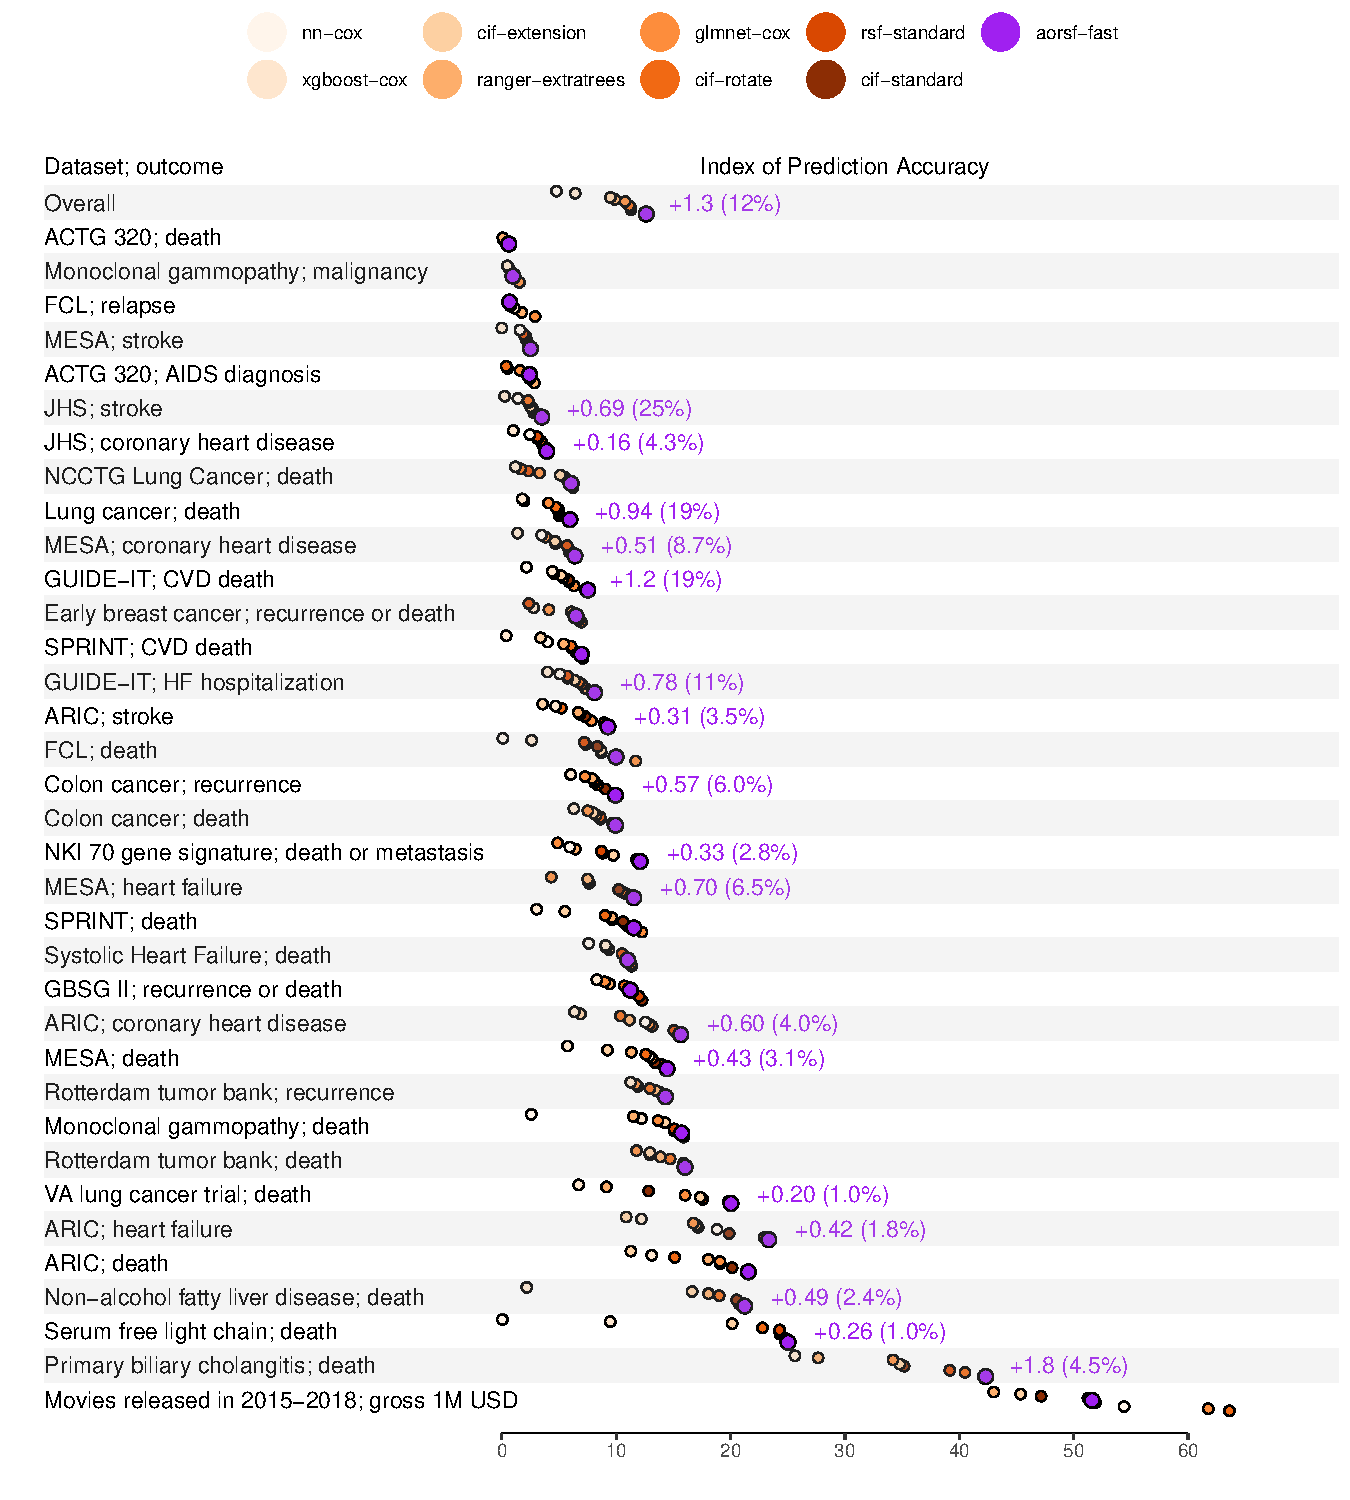
\includegraphics[width=\maxwidth]{figure/bm_pred_viz_ibs-1} \caption[Index of prediction accuracy in multiple risk prediction tasks]{Index of prediction accuracy in multiple risk prediction tasks. Text appears in tasks where the accelerated oblique random survival forest obtained the highest score, showing absolute and relative improvement over the second best learner. Since this figure is intended to compare \texttt{aorsf-fast} to learners that are not oblique random survival forests, \texttt{aorsf-cph}, \texttt{aorsf-random}, and \texttt{obliqueRSF-net} are not included.}\label{fig:bm_pred_viz_ibs}
\end{figure}

\end{knitrout}


\begin{knitrout}
\definecolor{shadecolor}{rgb}{0.969, 0.969, 0.969}\color{fgcolor}\begin{figure}
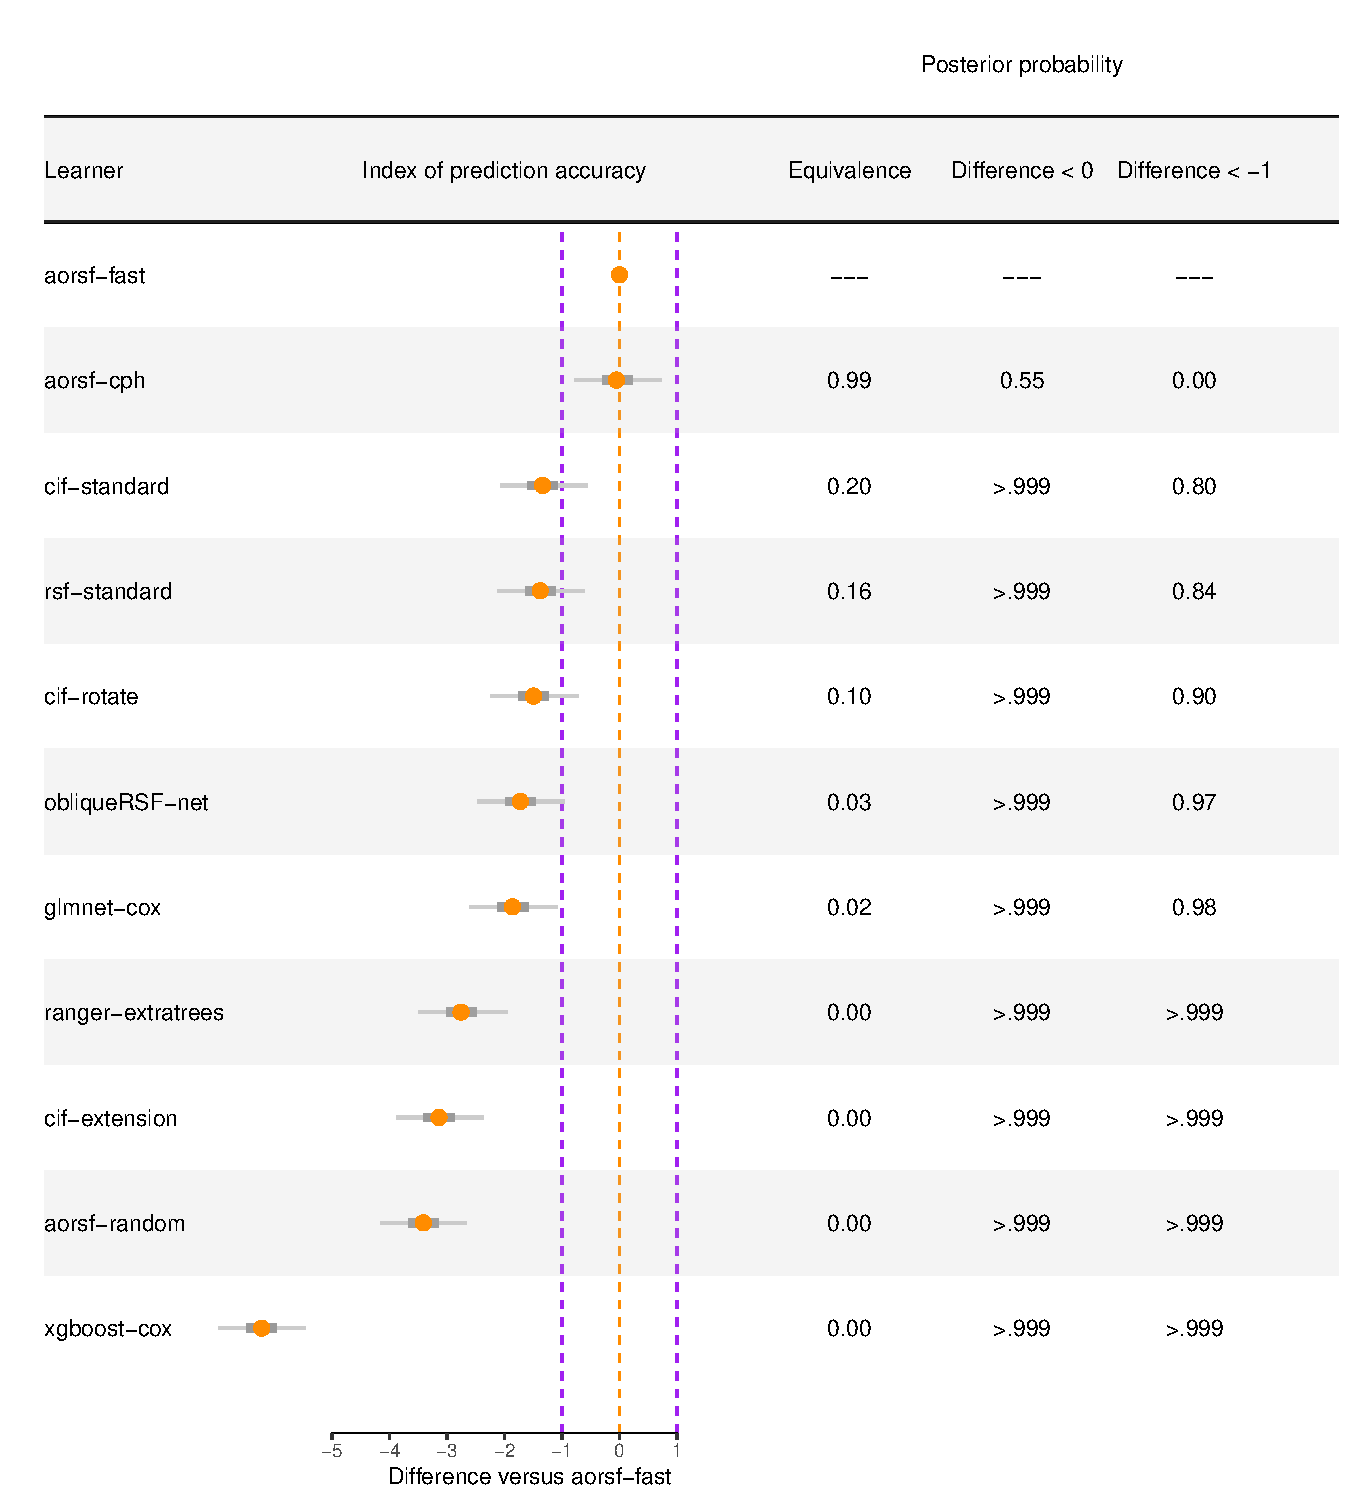
\includegraphics[width=\maxwidth]{figure/bm_pred_model_viz_ibs-1} \caption[Expected differences in index of prediction accuracy between the accelerated oblique random survival forest and other learning algorithms]{Expected differences in index of prediction accuracy between the accelerated oblique random survival forest and other learning algorithms. A region of practical equivalence is shown by purple dotted lines, and a boundary of non-zero difference is shown by an orange dotted line at the origin.}\label{fig:bm_pred_model_viz_ibs}
\end{figure}

\end{knitrout}

\paragraph{Time-dependent concordance statistic}




Compared to learners that were not oblique RSFs, \texttt{aorsf-fast} had the highest time-dependent C-statistic in 9 out of 35 risk prediction tasks, with an overall mean of 77.2 (Figure \ref{fig:bm_pred_viz_cstat}). Compared to the learner with the second highest mean C-statistic (\texttt{cif-standard}), \texttt{aorsf-fast}'s mean was 0.668 points higher, a relative increase of 0.873\%. The posterior probability of \texttt{aorsf-fast} and \texttt{aorsf-cph} having practically equivalent expected time-dependent C-statistics was $>$ 0.999, and the posterior probability of \texttt{aorsf-fast} having a superior time-dependent C-statistic versus other learners ranged from 0.15 (versus \texttt{cif-standard}) to $>$0.999 (versus several other learners; see Figure \ref{fig:bm_pred_model_viz_cstat})

\begin{knitrout}
\definecolor{shadecolor}{rgb}{0.969, 0.969, 0.969}\color{fgcolor}\begin{figure}
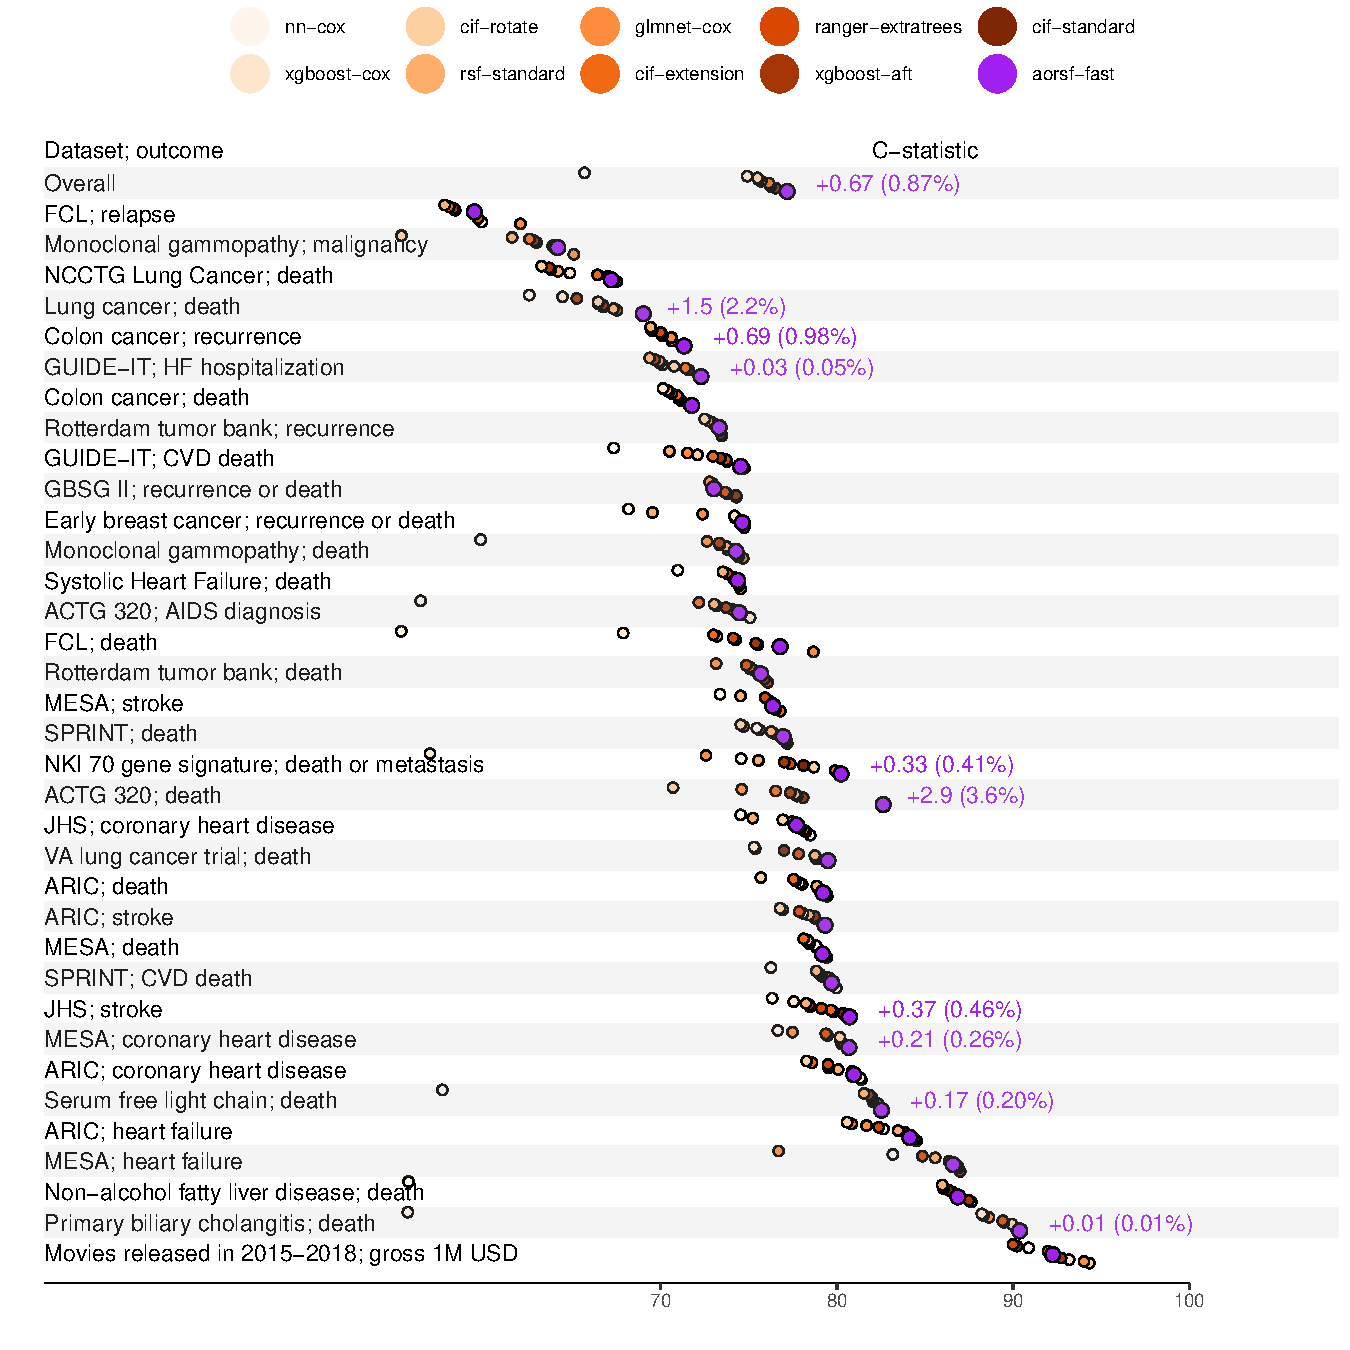
\includegraphics[width=\maxwidth]{figure/bm_pred_viz_cstat-1} \caption[Time-dependent concordance statistic for the accelerated oblique random survival forest and other learning algorithms across multiple risk prediction tasks]{Time-dependent concordance statistic for the accelerated oblique random survival forest and other learning algorithms across multiple risk prediction tasks. Text appears in tasks where the accelerated oblique random survival forest obtained the highest concordance, showing the absolute and percent improvement over the second best learner. Since this figure is intended to compare \texttt{aorsf-fast} to learners that are not oblique random survival forests, \texttt{aorsf-cph}, \texttt{aorsf-random}, and \texttt{obliqueRSF-net} are not included.}\label{fig:bm_pred_viz_cstat}
\end{figure}

\end{knitrout}


\begin{knitrout}
\definecolor{shadecolor}{rgb}{0.969, 0.969, 0.969}\color{fgcolor}\begin{figure}
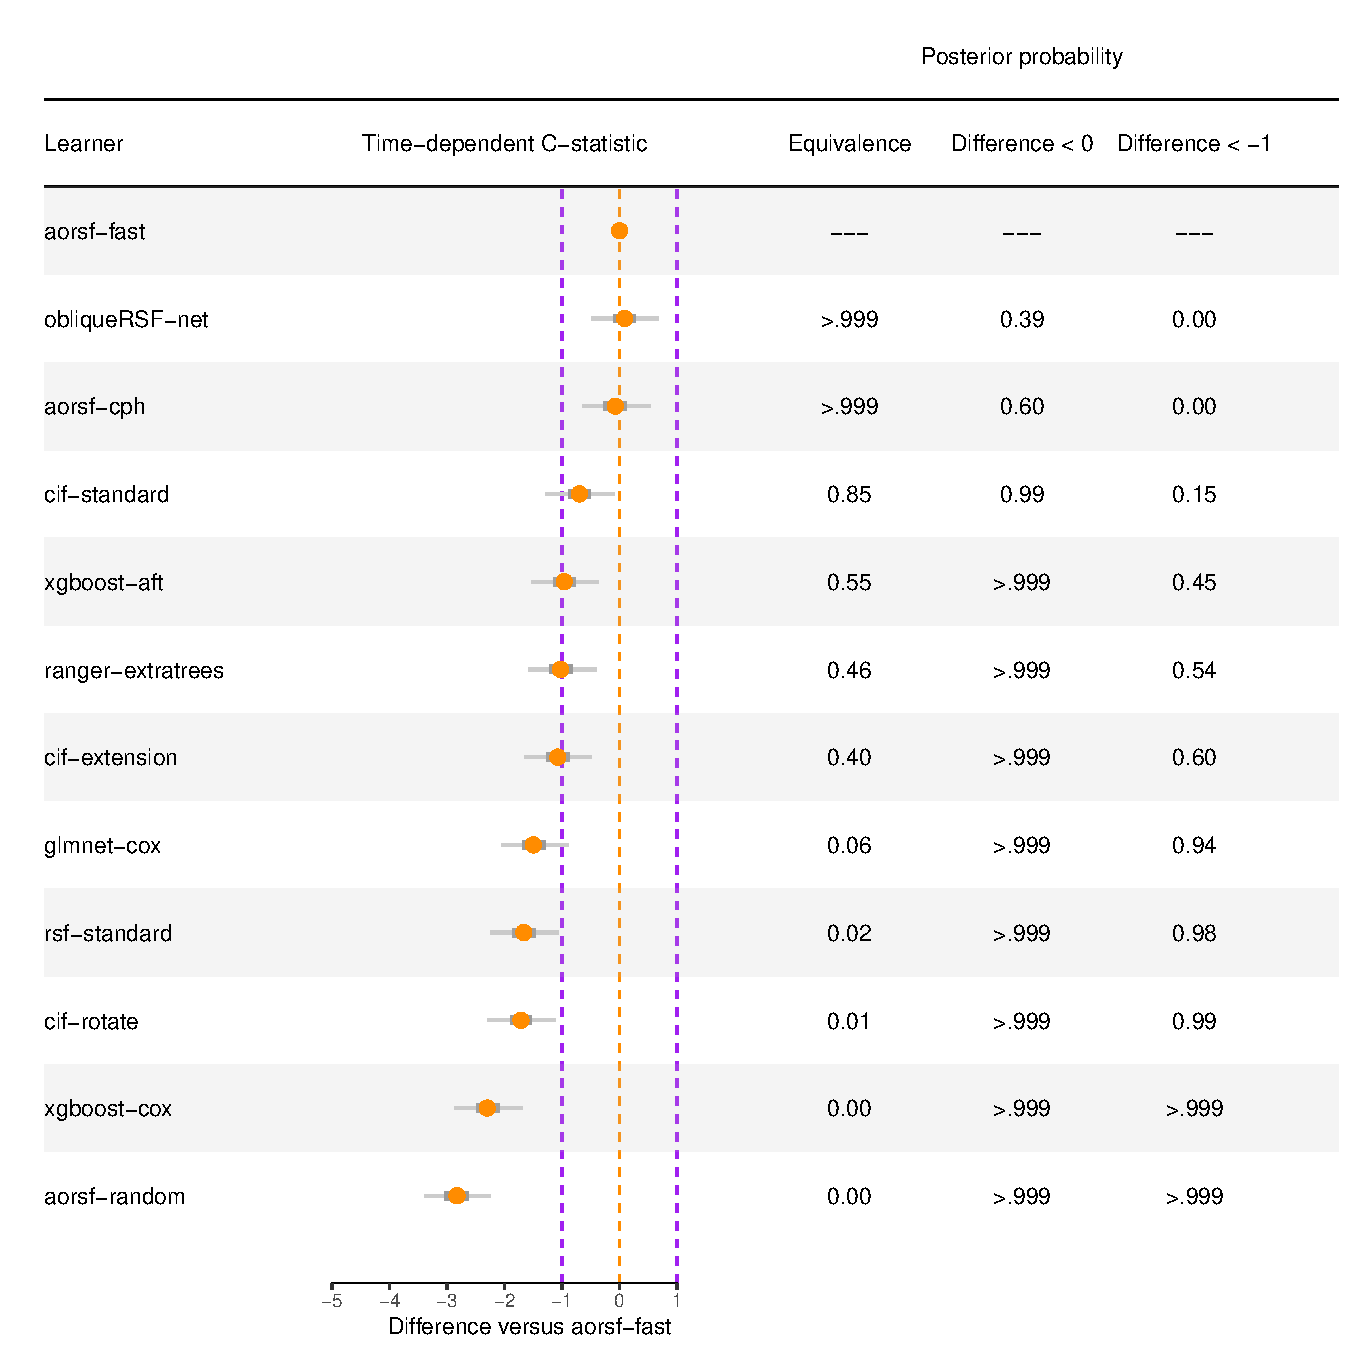
\includegraphics[width=\maxwidth]{figure/bm_pred_model_viz_cstat-1} \caption[Expected differences in time-dependent concordance statistic between the accelerated oblique random survival forest and other learning algorithms]{Expected differences in time-dependent concordance statistic between the accelerated oblique random survival forest and other learning algorithms. A region of practical equivalence is shown by purple dotted lines, and a boundary of non-zero difference is shown by an orange dotted line at the origin.}\label{fig:bm_pred_model_viz_cstat}
\end{figure}

\end{knitrout}

\subsection{Variable importance} \label{sec:results_vi}



The three techniques that used `aorsf' to estimate VI were ranked first (\texttt{aorsf-negate}; $C = 75.9$), second (\texttt{aorsf-anova}; $C = 73.9$), and third (\texttt{aorsf-permute}; $C = 73.2$) in overall mean C-statistic across all of the simulation scenarios, with \texttt{aorsf-negate} obtaining the highest C-statistic in 26 out of 36 VI tasks (Figure \ref{fig:bm_vi_viz}). Among the four relevant variable classes, \texttt{aorsf-negate} had the highest mean C-statistic for main effects, combination effects, and non-linear effects, with the greatest advantage of using \texttt{aorsf-negate} occurring among non-linear and combination variables. Full results from the experiment are provided in \tabrefAppendix{tab:bm_vi} in Supplementary Materials. Computationally, ANOVA VI was faster than negation and permutation VI, with a median time of 2.88 seconds versus 20.4 and 21.8 seconds, respectively.

\begin{knitrout}
\definecolor{shadecolor}{rgb}{0.969, 0.969, 0.969}\color{fgcolor}\begin{figure}
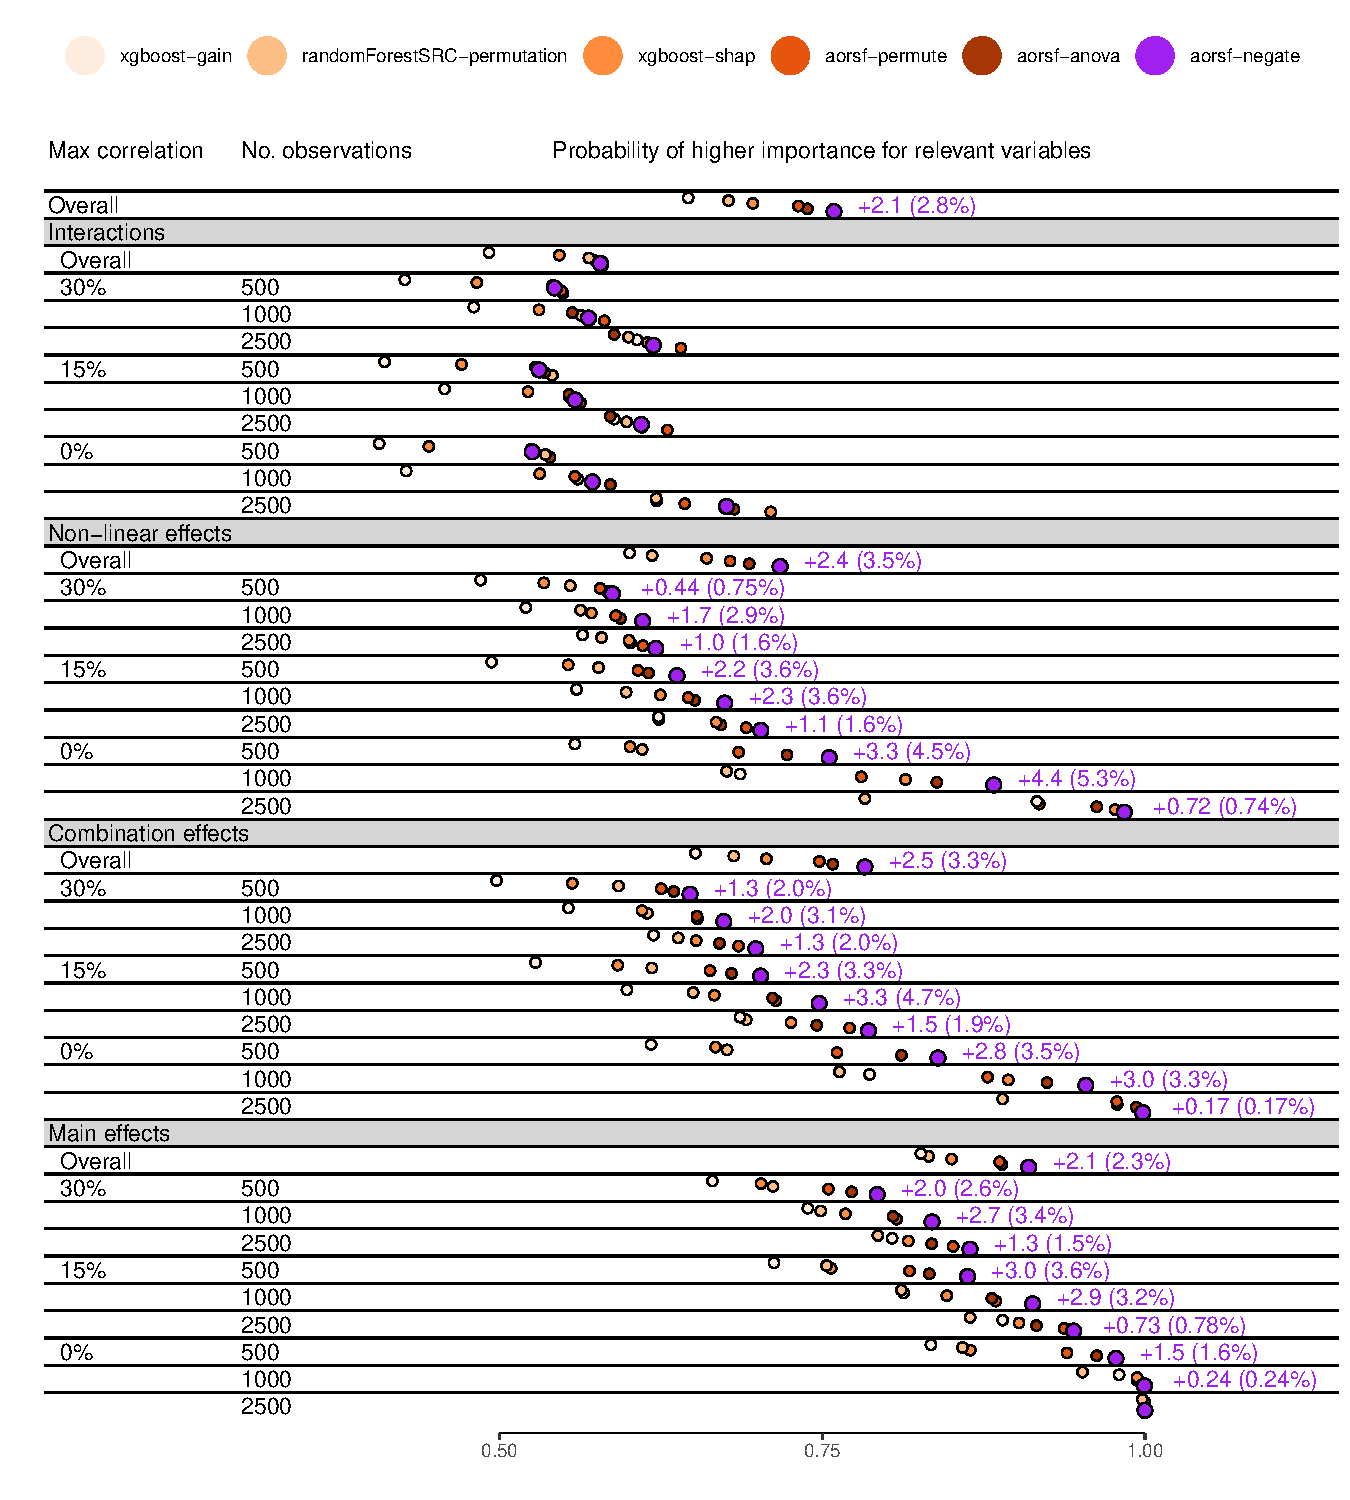
\includegraphics[width=\maxwidth]{figure/bm_vi_viz-1} \caption[Concordance statistic for assigning higher importance to relevant versus irrelevant variables]{Concordance statistic for assigning higher importance to relevant versus irrelevant variables. Text appears in rows where negation importance obtained the highest concordance, showing absolute and percent improvement over the second best technique.}\label{fig:bm_vi_viz}
\end{figure}

\end{knitrout}

\subsection{Computational efficiency} \label{sec:results_computing}




In the analysis of 35 risk prediction tasks, \texttt{aorsf-fast} was the second fastest learner overall, with a median time to develop a risk prediction model and compute predictions about 337 milliseconds longer than \texttt{glmnet-cox} (Figure \ref{fig:bm_pred_time}). Comparing median computing times, \texttt{aorsf-fast} was 1,291.6 times faster than its predecessor, \texttt{obliqueRSF-net}. In addition, \texttt{aorsf-fast} was 19.8, 1.90, and 3.18 faster than axis based forests grown using the \texttt{party}, \texttt{ranger}, and \texttt{randomForestSRC} packages, respectively.

\begin{knitrout}
\definecolor{shadecolor}{rgb}{0.969, 0.969, 0.969}\color{fgcolor}\begin{figure}
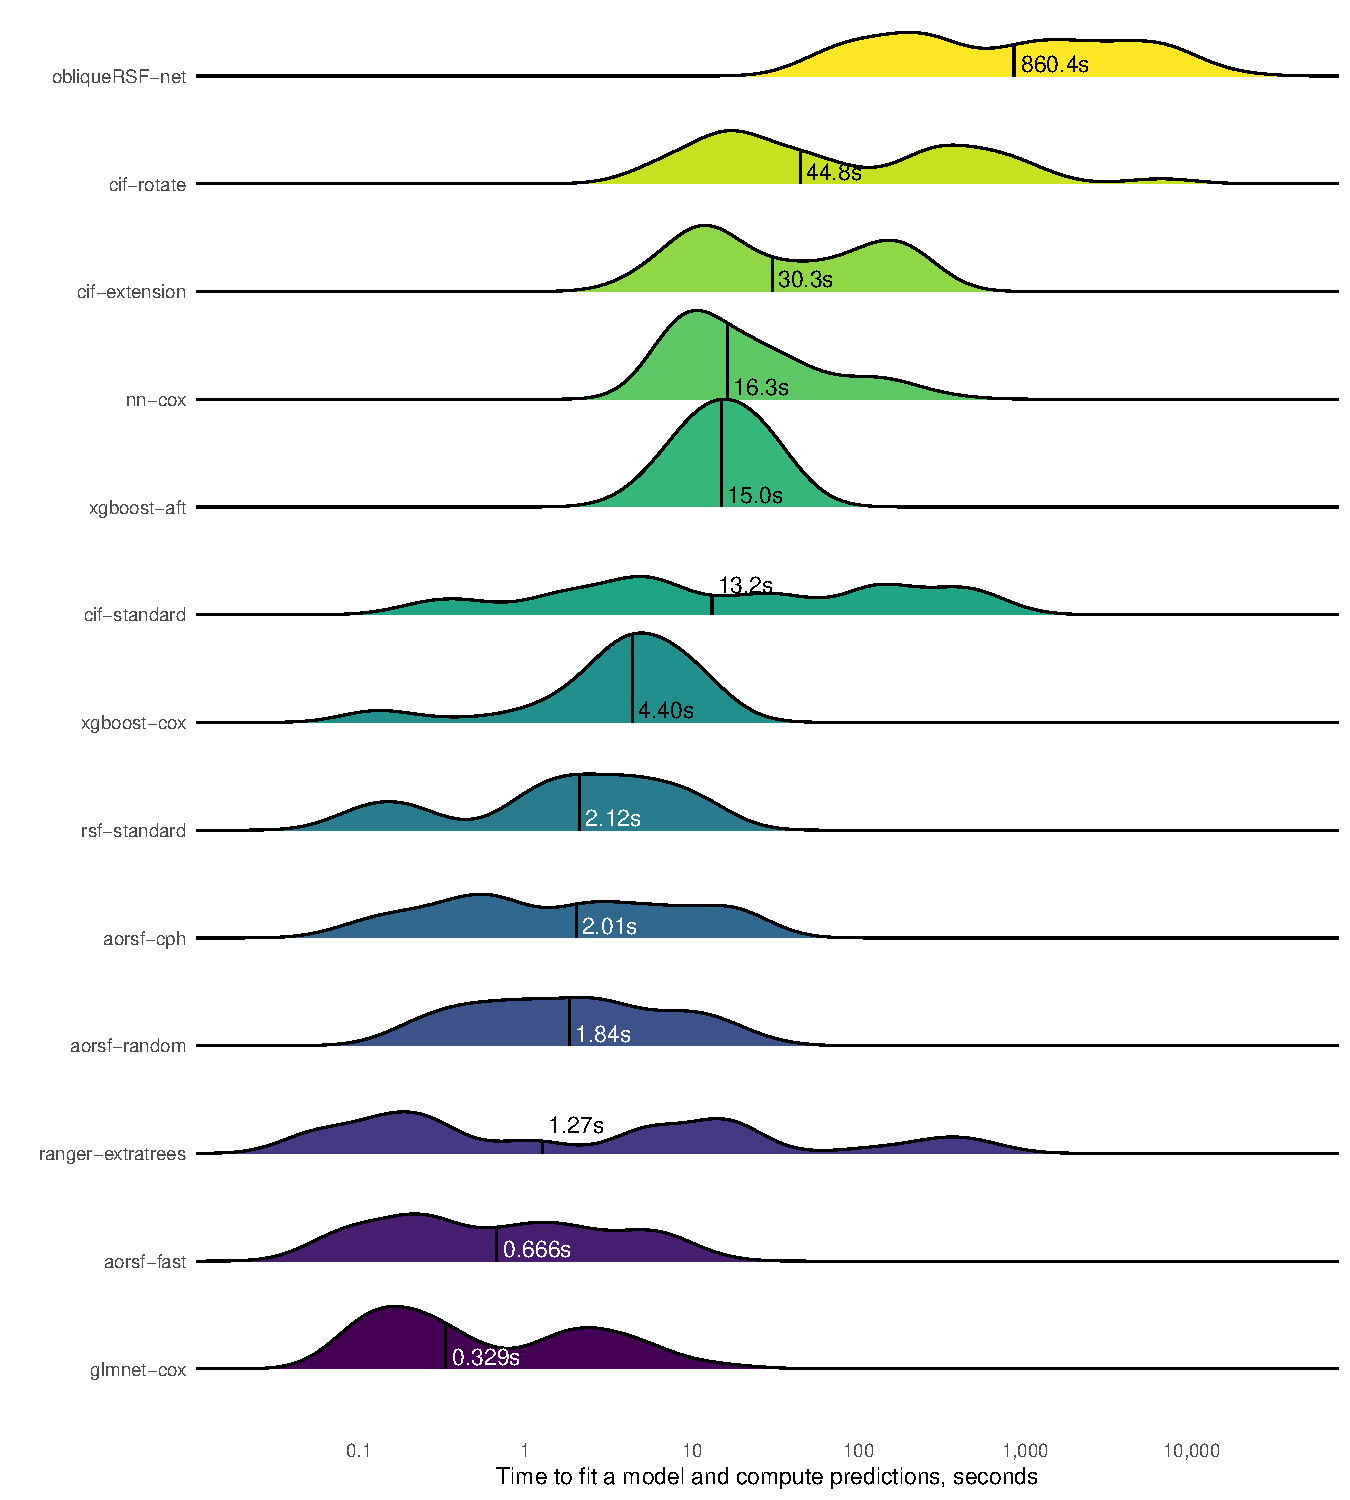
\includegraphics[width=\maxwidth]{figure/bm_pred_time-1} \caption[Distribution of time taken to fit a prediction model and compute predicted risk]{Distribution of time taken to fit a prediction model and compute predicted risk. The median time, in seconds, is printed and annotated for each learner by a vertical line.}\label{fig:bm_pred_time}
\end{figure}

\end{knitrout}

In the analysis of time to fit 500 trees using simulated data, the \texttt{ranger} package exhibited the fastest computation times overall (Figure \ref{fig:bm_time_viz}). \texttt{aorsf} was the second fastest when the number of predictors was 10 or 100,  and \texttt{randomForestSRC} had similar computation time versus \texttt{aorsf} when 1000 predictors were present.

\begin{knitrout}
\definecolor{shadecolor}{rgb}{0.969, 0.969, 0.969}\color{fgcolor}\begin{figure}
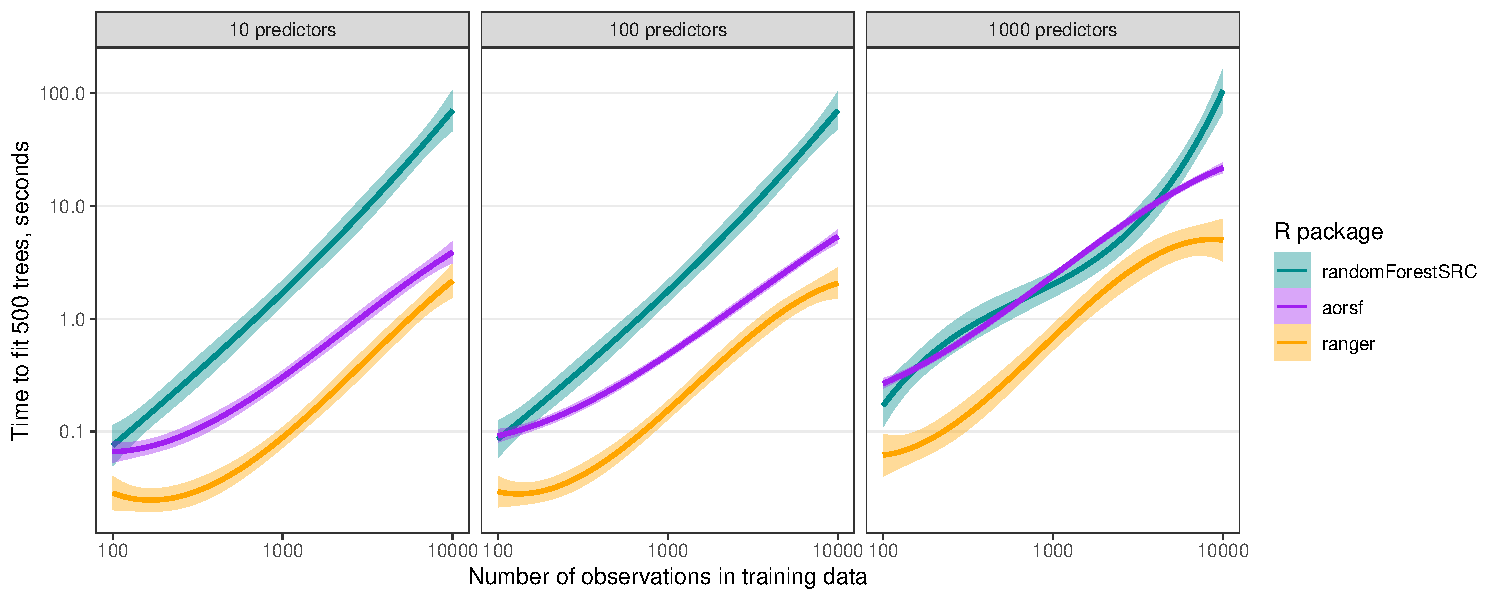
\includegraphics[width=\maxwidth]{figure/bm_time_viz-1} \caption[The expected time, in seconds, to fit an ensemble of 500 axis-based survival trees using the ranger or randomForestSRC package versus 500 oblique survival trees using the aorsf package]{The expected time, in seconds, to fit an ensemble of 500 axis-based survival trees using the ranger or randomForestSRC package versus 500 oblique survival trees using the aorsf package. The ranger package is the most efficient overall, and aorsf appears to be relatively efficient in larger samples, particularly when 10 or 100 predictors are present in the training data. All three packages appear to scale linearly in computation time with the number of observations in the training data.}\label{fig:bm_time_viz}
\end{figure}

\end{knitrout}


\section{Discussion} \label{sec:discussion}

In this paper, we have developed two contributions to the oblique RSF: (1) the accelerated oblique RSF (\ie, \texttt{aorsf-fast}) and (2) negation VI. Our technique to accelerate the oblique RSF reduces the number of operations required to find linear combinations of inputs using a single iteration of Newton Raphson scoring, while our VI technique directly engages with coefficients in linear combinations of inputs to measure importance of individual variables. In numeric experiments, we found that \texttt{aorsf-fast} is approximately 1,291.6 times faster than its predecessor, \texttt{obliqueRSF-net}, with a practically equivalent C-statistic. We also found that negation VI, a technique to estimate VI using the oblique RSF, detected non-linear, combination, and main effects more effectively than three standard methods to estimate VI: permutation, ANOVA, and SHAP VI. Overall, we found that estimating VI using negation instead of ANOVA increased the C-statistic for ranking a relevant variable higher than an irrelevant variable by 2.05, a relative increase of 2.78\%.

To understand potential differences in computational efficiency, we reviewed code in the \texttt{aorsf}, \texttt{randomForestSRC}, and \texttt{ranger} packages. We found differences in how survival outcome data are saved in leaf nodes. For each leaf node, \texttt{aorsf} stores data with one row per unique event time using training data that are stored in the leaf, whereas \texttt{randomForestSRC} and \texttt{ranger} store survival outcomes at a fixed grid of event times in each leaf. By default, \texttt{ranger} creates a grid that includes all event times in the training data. The grid strategy can cause higher computing time and memory usage when the grid of event times is large and a large number of leaf nodes are included in each tree, which can occur when minimum node size is small relative to the size of the training data. We kept minimum node size fixed in our benchmark of computational efficiency using real data, and dymanically increased minimum node size based on the size of the training set when we benchmarked computational efficiency using simulated data. Because of this decision, the \texttt{randomForestSRC} and \texttt{ranger} packages ran slower than \texttt{aorsf} in our benchmark of real data but not in the benchmark of simulated data.

\subsection{Implications of our results}

Accurate risk prediction models have the potential to improve healthcare by directing timely interventions to patients who are most likely to benefit. However, prediction models that cannot scale adequately to large databases or cannot be interpreted and explained will struggle to gain acceptance in clinical practice \citep{moss2022demystifying}. The current study advances the oblique RSF, an accurate risk prediction model, towards being accurate, scalable, and interpretable. The improved computational efficiency of the accelerated oblique RSF increases the feasibility of applying oblique RSFs in a wide range of prediction tasks. Faster model evaluation and re-fitting also improve diagnosis and resolution of model-based issues (\eg, model calibration deteriorates over time). The introduction of negation VI also advances interpretability. VI is intrinsically linked to model fairness, as it can be used to identify when protected characteristics such as race, religion, and sexuality are inadvertently used (either directly or through correlates of these characteristics) by a prediction model. Since negation VI engages with the coefficients used in linear combinations of variables, a major component of oblique RSFs, it may be more capable of diagnosing unfairness in oblique RSFs compared to permutation importance and model-agnostic VI techniques.

\subsection{Limitations and next steps}

While the current study advances the oblique RSF towards being scalable and interpretable, there remain several limitations that can be targeted in future studies. The validity of the Cox partial likelihood function depends on an assumption of non-informative censoring, therefore the oblique RSF could be improved by incorporating methods to account for informative censoring prior to identifying a linear combination of variables \citep{he2016proportional, cui2017consistency}.  The accelerated oblique RSF does not account for competing risks, and biased estimation of incidence may occur when competing risks are ignored. Thus, allowing the oblique RSF to account for competing risks is a high priority for future studies. In addition, the current study only considered data without missing values, only evaluated oblique RSFs that applied the log-rank statistic for node splitting, and only considered negation VI estimates based on Harrell's C-statistic. Few studies have developed strategies to deal with missing data while growing oblique survival trees. Prior studies have found that log-rank tests can be mis-informative when survival curves cross \citep{li2015statistical}, and that Harrell's C-statistic is dependent on the censoring distribution of the outcome \citep{uno2011c}. Thus, a second item is to expand the range of options available to users of the \texttt{aorsf} package, enabling them to apply strategies for imputation of missing values and use a broad range of statistical criteria while growing oblique survival trees. Last, \citet{cui2017consistency} found that estimating an inverse-probability weighted hazard function at each non-leaf node of a survival tree allows the RSF to converge asymptotically to the true survival function when some variables contribute both to the risk of the event and the risk of censoring, a scenario that is very likely in the analysis of medical data. The accelerated oblique RSF could incorporate this splitting technique by using Newton Raphson scoring to fit a model for the censoring distribution after which a weighted model could be fit to the failure distribution. This final item has the highest priority, as \citet{cui2017consistency} showed it is a requisite condition for consistency of axis-based survival trees in fairly general settings.

% Acknowledgements should go at the end, before appendices and references

\subsection{Conclusion}

Oblique RSFs have exceptional prediction accuracy and this study has shown how they can be fit with computational efficiency that rivals their axis-based counterparts. We have also introduced a general and flexible method to estimate VI with oblique RFs, and demonstrated its effectiveness for numeric, correlated predictors.

\section{Supplementary Materials}

Supplemental materials for the current analysis are available online.

\begin{description}

\item[Code] The code used to generate results in the current analysis are available online at \newline https://github.com/bcjaeger/aorsf-bench and provided as supplemental material (aorsf\_bench.zip).

\item[aorsf] The R package used to fit oblique RSFs in the current analysis is available online at \newline https://github.com/ropensci/aorsf and version 0.0.7.9000 is provided as supplemental material (aorsf\_package.zip).

\item[Appendix] Additional details on data used in the current analysis as well as additional details for numeric experiments (aorsf\_appendix.pdf).

\end{description}

\bibliographystyle{Chicago}

\bibliography{main}

\newpage

\appendix

\section*{Appendix}
\captionsetup{labelformat=AppendixTables}
\setcounter{table}{0}

\subsection*{Data sources}




\begin{enumerate}

 \item The ``VA lung cancer trial'' data \citep{kalbfleisch2011statistical} were obtained from the \texttt{randomForestSRC} R package \citep{randomForestSRC}. No relevant pre-processing steps were taken. 
 \item The ``Colon cancer'' data \citep{moertel1995fluorouracil} were obtained from the \texttt{survival} R package \citep{survival}. In pre-processing steps, the predictor, node4, which is an indicator for having more than 4 positive lymph nodes, was dropped, while the nodes predictor, which indicates the number of positive lymph nodes, was retained. 
 \item The ``Primary biliary cholangitis'' data \citep{therneau2000cox} were obtained from the \texttt{aorsf} R package \citep{aorsf}. No relevant pre-processing steps were taken. 
 \item The ``Movies released in 2015-2018'' data  were obtained from the \texttt{censored} R package \citep{censored}. In pre-processing steps, text and date variables (movie title, release date, and distributor) were dropped.. 
 \item The ``GBSG II'' data \citep{schumacher1994rauschecker} were obtained from the \texttt{TH.data} R package \citep{TH.data}. No relevant pre-processing steps were taken. 
 \item The ``Systolic Heart Failure'' data \citep{hsich2011identifying} were obtained from the \texttt{randomForestSRC} R package \citep{randomForestSRC}. No relevant pre-processing steps were taken. 
 \item The ``Serum free light chain'' data \citep{dispenzieri2012use, kyle2006prevalence} were obtained from the \texttt{survival} R package \citep{survival}. In pre-processing steps, the chapter variable, which indicates death status, was removed, since death was the outcome. Outcomes occurring on day 0 were assumed to have a time of 1/2 day rather than 0 days. 
 \item The ``Non-alcohol fatty liver disease'' data \citep{allen2018nonalcoholic} were obtained from the \texttt{survival} R package \citep{survival}. In pre-processing steps, data from before or on the index data were used as predictors. The mean value prior to the index date for lab values in nafld2 was used as a predictor, and the number of days between the most recent lab test and the index date was also used as a predictor. 
 \item The ``Rotterdam tumor bank'' data \citep{royston2013external} were obtained from the \texttt{survival} R package \citep{survival}. No relevant pre-processing steps were taken. 
 \item The ``ACTG 320'' data \citep{hosmer2002applied} were obtained from the \texttt{mlr3proba} R package \citep{mlr3proba}. In pre-processing steps, redundant predictors were dropped. 
 \item The ``GUIDE-IT'' data \citep{felker2017effect} were obtained from BioLINCC. In pre-processing steps, baseline data including biomarkers, questionnaires, and randomized group were included as predictors. 
 \item The ``Early breast cancer'' data \citep{desmedt2011multifactorial, hatzis2011genomic, ternes2017identification} were obtained from the \texttt{biospear} R package \citep{biospear}. No relevant pre-processing steps were taken. 
 \item The ``SPRINT'' data \citep{sprint2015randomized} were obtained from BioLINCC. In pre-processing steps, baseline data including biomarkers, cognitive questionnaires, medications, and randomization group were included as predictors. Predictors with over 40 percent missing data were dropped. Zero variance predictors were also dropped. 
 \item The ``NKI 70 gene signature'' data \citep{van2002gene} were obtained from the \texttt{OpenML} R package \citep{OpenML}. No relevant pre-processing steps were taken. 
 \item The ``Lung cancer'' data \citep{director2008gene} were obtained from the \texttt{OpenML} R package \citep{OpenML}. In pre-processing steps, status was transformed to have values of 0 and 1 instead of 1 and 2. 
 \item The ``NCCTG Lung Cancer'' data \citep{loprinzi1994prospective} were obtained from the \texttt{survival} R package \citep{survival}. In pre-processing steps, institution code was not used as a predictor, and values of both sex and event status were transformed to be 0 and 1 instead of 1 and 2. 
 \item The ``FCL'' data \citep{pintilie2006competing} were obtained from the \texttt{randomForestSRC} R package \citep{randomForestSRC}. No relevant pre-processing steps were taken. 
 \item The ``Monoclonal gammopathy'' data \citep{kyle2002long} were obtained from the \texttt{survival} R package \citep{survival}. No relevant pre-processing steps were taken. 
 \item The ``MESA'' data \citep{bild2002multi} were obtained from BioLINCC. In pre-processing steps, visit 1 data including biomarkers, health behaviors, and comorbidities were included as predictors. 
 \item The ``ARIC'' data \citep{aric1989atherosclerosis} were obtained from BioLINCC. In pre-processing steps, visit 1 data including biomarkers, health behaviors, and comorbidities were included as predictors. 
 \item The ``JHS'' data \citep{taylor2005toward} were obtained from BioLINCC. In pre-processing steps, visit 1 data including biomarkers, health behaviors, neighborhood characteristics, and comorbidities were included as predictors.

\end{enumerate}

\begin{knitrout}
\definecolor{shadecolor}{rgb}{0.969, 0.969, 0.969}\color{fgcolor}
\begin{landscape}
\begin{longtable}[t]{lcclcc}
\caption{\label{tab:unnamed-chunk-10}Data sets used for numeric experiments \label{tab:datasets}}\\
\toprule
Label & N observations & N predictors & Outcome & N Events & \% Censored\\
\midrule
VA lung cancer trial & 137 & 8 & Death & 128 & 6.57\\
\cmidrule{1-6}\pagebreak[0]
 &  &  & Recurrence & 468 & 49.6\\
\cmidrule{4-6}\nopagebreak
\multirow{-2}{*}{\raggedright\arraybackslash Colon cancer} & \multirow{-2}{*}{\centering\arraybackslash 929} & \multirow{-2}{*}{\centering\arraybackslash 12} & Death & 452 & 51.3\\
\cmidrule{1-6}\pagebreak[0]
Primary biliary cholangitis & 276 & 19 & Death & 111 & 59.8\\
\cmidrule{1-6}\pagebreak[0]
Movies released in 2015-2018 & 551 & 46 & Gross 1M USD & 522 & 5.26\\
\cmidrule{1-6}\pagebreak[0]
GBSG II & 686 & 10 & Recurrence Or Death & 299 & 56.4\\
\cmidrule{1-6}\pagebreak[0]
Systolic Heart Failure & 2,231 & 41 & Death & 726 & 67.5\\
\cmidrule{1-6}\pagebreak[0]
Serum free light chain & 7,874 & 10 & Death & 2,169 & 72.5\\
\cmidrule{1-6}\pagebreak[0]
Non-alcohol fatty liver disease & 17,549 & 24 & Death & 1,364 & 92.2\\
\cmidrule{1-6}\pagebreak[0]
 &  &  & Recurrence & 1,518 & 49.1\\
\cmidrule{4-6}\nopagebreak
\multirow{-2}{*}{\raggedright\arraybackslash Rotterdam tumor bank} & \multirow{-2}{*}{\centering\arraybackslash 2,982} & \multirow{-2}{*}{\centering\arraybackslash 11} & Death & 1,272 & 57.3\\
\cmidrule{1-6}\pagebreak[0]
 &  &  & AIDS Diagnosis & 96 & 91.7\\
\cmidrule{4-6}\nopagebreak
\multirow{-2}{*}{\raggedright\arraybackslash ACTG 320} & \multirow{-2}{*}{\centering\arraybackslash 1,151} & \multirow{-2}{*}{\centering\arraybackslash 12} & Death & 26 & 97.7\\
\cmidrule{1-6}\pagebreak[0]
 &  &  & Cardiovascular Death & 110 & 87.7\\
\cmidrule{4-6}\nopagebreak
\multirow{-2}{*}{\raggedright\arraybackslash GUIDE-IT} & \multirow{-2}{*}{\centering\arraybackslash 894} & \multirow{-2}{*}{\centering\arraybackslash 59} & Hf Hospitalization & 288 & 67.8\\
\cmidrule{1-6}\pagebreak[0]
Early breast cancer & 614 & 1,692 & Recurrence Or Death & 134 & 78.2\\
\cmidrule{1-6}\pagebreak[0]
 &  &  & Cardiovascular Death & 521 & 94.4\\
\cmidrule{4-6}\nopagebreak
\multirow{-2}{*}{\raggedright\arraybackslash SPRINT} & \multirow{-2}{*}{\centering\arraybackslash 9,361} & \multirow{-2}{*}{\centering\arraybackslash 174} & Death & 1,644 & 82.4\\
\cmidrule{1-6}\pagebreak[0]
NKI 70 gene signature & 144 & 77 & Death Or Metastasis & 48 & 66.7\\
\cmidrule{1-6}\pagebreak[0]
Lung cancer & 442 & 24 & Death & 236 & 46.6\\
\cmidrule{1-6}\pagebreak[0]
NCCTG Lung Cancer & 228 & 9 & Death & 165 & 27.6\\
\cmidrule{1-6}\pagebreak[0]
 &  &  & Death & 76 & 86.0\\
\cmidrule{4-6}\nopagebreak
\multirow{-2}{*}{\raggedright\arraybackslash FCL} & \multirow{-2}{*}{\centering\arraybackslash 541} & \multirow{-2}{*}{\centering\arraybackslash 7} & Relapse & 272 & 49.7\\
\cmidrule{1-6}\pagebreak[0]
 &  &  & Death & 963 & 30.4\\
\cmidrule{4-6}\nopagebreak
\multirow{-2}{*}{\raggedright\arraybackslash Monoclonal gammopathy} & \multirow{-2}{*}{\centering\arraybackslash 1,384} & \multirow{-2}{*}{\centering\arraybackslash 8} & Malignancy & 115 & 91.7\\
\cmidrule{1-6}\pagebreak[0]
 &  &  & Heart Failure & 339 & 95.0\\
\cmidrule{4-6}\nopagebreak
 &  &  & Coronary Heart Disease & 439 & 93.5\\
\cmidrule{4-6}\nopagebreak
 &  &  & Stroke & 292 & 95.7\\
\cmidrule{4-6}\nopagebreak
\multirow{-4}{*}{\raggedright\arraybackslash MESA} & \multirow{-4}{*}{\centering\arraybackslash 6,783} & \multirow{-4}{*}{\centering\arraybackslash 48} & Death & 1,297 & 80.9\\
\cmidrule{1-6}\pagebreak[0]
 &  &  & Heart Failure & 2,981 & 78.1\\
\cmidrule{4-6}\nopagebreak
 &  &  & Coronary Heart Disease & 2,282 & 83.2\\
\cmidrule{4-6}\nopagebreak
 &  &  & Stroke & 1,323 & 90.3\\
\cmidrule{4-6}\nopagebreak
\multirow{-4}{*}{\raggedright\arraybackslash ARIC} & \multirow{-4}{*}{\centering\arraybackslash 13,623} & \multirow{-4}{*}{\centering\arraybackslash 41} & Death & 6,662 & 51.1\\
\cmidrule{1-6}\pagebreak[0]
 &  &  & Stroke & 152 & 95.8\\
\cmidrule{4-6}\nopagebreak
\multirow{-2}{*}{\raggedright\arraybackslash JHS} & \multirow{-2}{*}{\centering\arraybackslash 3,501} & \multirow{-2}{*}{\centering\arraybackslash 80} & Coronary Heart Disease & 190 & 94.6\\
\bottomrule
\end{longtable}
\end{landscape}

\end{knitrout}

\newpage

\begin{knitrout}
\definecolor{shadecolor}{rgb}{0.969, 0.969, 0.969}\color{fgcolor}
\begin{longtable}[t]{lcccc}
\caption{\label{tab:unnamed-chunk-11}Index of prediction accuracy, time-dependent concordance statistic, and computational time required to fit and compute predictions for several learning algorithms across 35 risk prediction tasks.\label{tab:bm_pred_all}}\\
\toprule
\multicolumn{1}{c}{ } & \multicolumn{2}{c}{Performance metric (SD)} & \multicolumn{2}{c}{Computation time, seconds} \\
\cmidrule(l{3pt}r{3pt}){2-3} \cmidrule(l{3pt}r{3pt}){4-5}
  & Scaled Brier & C-Statistic & Model fitting & Risk prediction\\
\midrule
\endfirsthead
\caption[]{Index of prediction accuracy, time-dependent concordance statistic, and computational time required to fit and compute predictions for several learning algorithms across 35 risk prediction tasks.\label{tab:bm_pred_all} \textit{(continued)}}\\
\toprule
  & Scaled Brier & C-Statistic & Model fitting & Risk prediction\\
\midrule
\endhead

\endfoot
\bottomrule
\endlastfoot
\addlinespace[0.3em]
\multicolumn{5}{l}{\textit{\textbf{Overall}}}\\
\hline
\hspace{1em}aorsf-fast & 0.126 (0.109) & 0.772 (0.071) & 0.527 & 0.138\\
\hspace{1em}aorsf-cph & 0.126 (0.109) & 0.771 (0.070) & 1.750 & 0.140\\
\hspace{1em}cif-standard & 0.113 (0.098) & 0.765 (0.071) & 3.792 & 6.448\\
\hspace{1em}rsf-standard & 0.113 (0.114) & 0.755 (0.075) & 1.945 & 0.196\\
\hspace{1em}cif-rotate & 0.112 (0.124) & 0.755 (0.081) & 36.928 & 8.194\\
\hspace{1em}obliqueRSF-net & 0.109 (0.081) & 0.773 (0.069) & 552.335 & 84.685\\
\hspace{1em}glmnet-cox & 0.108 (0.119) & 0.757 (0.077) & 0.326 & 0.003\\
\hspace{1em}ranger-extratrees & 0.099 (0.085) & 0.762 (0.067) & 0.790 & 1.109\\
\hspace{1em}cif-extension & 0.095 (0.092) & 0.761 (0.072) & 21.977 & 6.922\\
\hspace{1em}aorsf-random & 0.092 (0.079) & 0.744 (0.065) & 1.717 & 0.149\\
\hspace{1em}xgboost-cox & 0.064 (0.100) & 0.749 (0.094) & 4.394 & 0.004\\
\hspace{1em}nn-cox & 0.048 (0.106) & 0.657 (0.136) & 11.377 & 1.705\\
\hspace{1em}xgboost-aft & --- & 0.762 (0.076) & 15.031 & 0.007\\
\addlinespace[0.3em]
\multicolumn{5}{l}{\textit{\textbf{ACTG 320; AIDS diagnosis, n = 1151, p = 12}}}\\
\hline
\hspace{1em}obliqueRSF-net & 0.029 (0.015) & 0.753 (0.037) & 115.320 & 18.196\\
\hspace{1em}ranger-extratrees & 0.028 (0.017) & 0.740 (0.036) & 0.086 & 0.133\\
\hspace{1em}aorsf-random & 0.027 (0.020) & 0.756 (0.036) & 0.465 & 0.035\\
\hspace{1em}cif-standard & 0.024 (0.031) & 0.744 (0.040) & 1.657 & 4.377\\
\hspace{1em}aorsf-cph & 0.024 (0.029) & 0.750 (0.042) & 0.436 & 0.036\\
\hspace{1em}aorsf-fast & 0.024 (0.028) & 0.745 (0.045) & 0.141 & 0.036\\
\hspace{1em}cif-extension & 0.023 (0.015) & 0.722 (0.038) & 9.010 & 4.189\\
\hspace{1em}glmnet-cox & 0.016 (0.030) & 0.746 (0.037) & 0.197 & 0.002\\
\hspace{1em}rsf-standard & 0.005 (0.041) & 0.730 (0.042) & 0.179 & 0.061\\
\hspace{1em}cif-rotate & 0.004 (0.040) & 0.731 (0.038) & 14.549 & 3.604\\
\hspace{1em}nn-cox & 0.000 (0.011) & 0.564 (0.101) & 7.755 & 0.811\\
\hspace{1em}xgboost-cox & -0.001 (0.052) & 0.751 (0.033) & 3.729 & 0.003\\
\hspace{1em}xgboost-aft & --- & 0.737 (0.035) & 11.383 & 0.006\\
\addlinespace[0.3em]
\multicolumn{5}{l}{\textit{\textbf{ACTG 320; death, n = 1151, p = 12}}}\\
\hline
\hspace{1em}aorsf-random & 0.008 (0.012) & 0.798 (0.073) & 0.285 & 0.024\\
\hspace{1em}obliqueRSF-net & 0.006 (0.009) & 0.821 (0.049) & 49.070 & 11.201\\
\hspace{1em}aorsf-fast & 0.006 (0.019) & 0.826 (0.057) & 0.088 & 0.020\\
\hspace{1em}aorsf-cph & 0.006 (0.018) & 0.818 (0.062) & 0.357 & 0.020\\
\hspace{1em}cif-extension & 0.001 (0.020) & 0.765 (0.066) & 8.283 & 3.478\\
\hspace{1em}ranger-extratrees & 0.001 (0.019) & 0.777 (0.069) & 0.041 & 0.122\\
\hspace{1em}xgboost-cox & -0.004 (0.004) & 0.500 (0.000) & 0.118 & 0.002\\
\hspace{1em}nn-cox & -0.004 (0.004) & 0.547 (0.128) & 7.487 & 0.717\\
\hspace{1em}cif-standard & -0.005 (0.025) & 0.781 (0.062) & 1.695 & 4.223\\
\hspace{1em}rsf-standard & -0.031 (0.051) & 0.776 (0.073) & 0.098 & 0.037\\
\hspace{1em}cif-rotate & -0.037 (0.049) & 0.707 (0.090) & 13.163 & 3.201\\
\hspace{1em}glmnet-cox & -0.065 (0.095) & 0.746 (0.098) & 0.286 & 0.002\\
\hspace{1em}xgboost-aft & --- & 0.774 (0.070) & 10.124 & 0.005\\
\addlinespace[0.3em]
\multicolumn{5}{l}{\textit{\textbf{ARIC; coronary heart disease, n = 13623, p = 41}}}\\
\hline
\hspace{1em}aorsf-fast & 0.156 (0.007) & 0.810 (0.007) & 4.590 & 1.434\\
\hspace{1em}aorsf-cph & 0.153 (0.006) & 0.809 (0.007) & 14.582 & 1.450\\
\hspace{1em}rsf-standard & 0.150 (0.007) & 0.801 (0.007) & 8.222 & 0.981\\
\hspace{1em}obliqueRSF-net & 0.133 (0.005) & 0.811 (0.008) & 4468.696 & 1359.275\\
\hspace{1em}cif-standard & 0.132 (0.005) & 0.809 (0.007) & 70.462 & 358.273\\
\hspace{1em}glmnet-cox & 0.129 (0.011) & 0.795 (0.008) & 1.873 & 0.010\\
\hspace{1em}nn-cox & 0.126 (0.012) & 0.795 (0.007) & 43.144 & 86.104\\
\hspace{1em}ranger-extratrees & 0.112 (0.005) & 0.795 (0.009) & 283.364 & 69.939\\
\hspace{1em}aorsf-random & 0.104 (0.005) & 0.771 (0.008) & 11.343 & 1.420\\
\hspace{1em}cif-rotate & 0.104 (0.004) & 0.783 (0.009) & 558.249 & 68.510\\
\hspace{1em}cif-extension & 0.069 (0.002) & 0.786 (0.009) & 164.161 & 50.420\\
\hspace{1em}xgboost-cox & 0.064 (0.017) & 0.813 (0.006) & 9.660 & 0.015\\
\hspace{1em}xgboost-aft & --- & 0.814 (0.006) & 29.321 & 0.013\\
\addlinespace[0.3em]
\multicolumn{5}{l}{\textit{\textbf{ARIC; death, n = 13623, p = 41}}}\\
\hline
\hspace{1em}rsf-standard & 0.216 (0.006) & 0.789 (0.004) & 12.352 & 1.162\\
\hspace{1em}aorsf-fast & 0.216 (0.006) & 0.792 (0.004) & 7.463 & 2.519\\
\hspace{1em}aorsf-cph & 0.215 (0.006) & 0.792 (0.004) & 22.389 & 2.569\\
\hspace{1em}cif-standard & 0.201 (0.004) & 0.790 (0.004) & 68.083 & 373.333\\
\hspace{1em}obliqueRSF-net & 0.195 (0.004) & 0.789 (0.004) & 7373.936 & 1276.463\\
\hspace{1em}nn-cox & 0.191 (0.008) & 0.779 (0.005) & 83.418 & 84.770\\
\hspace{1em}glmnet-cox & 0.191 (0.015) & 0.777 (0.007) & 2.282 & 0.011\\
\hspace{1em}ranger-extratrees & 0.181 (0.004) & 0.780 (0.005) & 356.276 & 61.525\\
\hspace{1em}cif-rotate & 0.151 (0.007) & 0.757 (0.006) & 563.575 & 64.849\\
\hspace{1em}xgboost-cox & 0.131 (0.012) & 0.794 (0.004) & 12.568 & 0.015\\
\hspace{1em}aorsf-random & 0.128 (0.006) & 0.725 (0.005) & 20.291 & 2.298\\
\hspace{1em}cif-extension & 0.113 (0.002) & 0.775 (0.005) & 176.867 & 50.345\\
\hspace{1em}xgboost-aft & --- & 0.794 (0.004) & 35.380 & 0.013\\
\addlinespace[0.3em]
\multicolumn{5}{l}{\textit{\textbf{ARIC; heart failure, n = 13623, p = 41}}}\\
\hline
\hspace{1em}aorsf-fast & 0.233 (0.006) & 0.841 (0.005) & 5.478 & 1.709\\
\hspace{1em}rsf-standard & 0.229 (0.006) & 0.835 (0.005) & 10.326 & 1.039\\
\hspace{1em}aorsf-cph & 0.229 (0.006) & 0.840 (0.005) & 17.063 & 1.730\\
\hspace{1em}cif-standard & 0.199 (0.005) & 0.839 (0.005) & 68.929 & 364.202\\
\hspace{1em}obliqueRSF-net & 0.198 (0.005) & 0.839 (0.005) & 5341.195 & 1624.560\\
\hspace{1em}nn-cox & 0.188 (0.018) & 0.826 (0.006) & 58.351 & 89.012\\
\hspace{1em}cif-rotate & 0.172 (0.006) & 0.806 (0.007) & 569.166 & 67.654\\
\hspace{1em}ranger-extratrees & 0.170 (0.004) & 0.824 (0.005) & 411.253 & 73.737\\
\hspace{1em}glmnet-cox & 0.167 (0.044) & 0.817 (0.018) & 2.257 & 0.010\\
\hspace{1em}aorsf-random & 0.151 (0.006) & 0.792 (0.007) & 14.023 & 1.686\\
\hspace{1em}xgboost-cox & 0.122 (0.017) & 0.845 (0.005) & 11.985 & 0.015\\
\hspace{1em}cif-extension & 0.109 (0.003) & 0.808 (0.006) & 169.620 & 49.957\\
\hspace{1em}xgboost-aft & --- & 0.844 (0.005) & 30.837 & 0.012\\
\addlinespace[0.3em]
\multicolumn{5}{l}{\textit{\textbf{ARIC; stroke, n = 13623, p = 41}}}\\
\hline
\hspace{1em}aorsf-fast & 0.093 (0.004) & 0.793 (0.007) & 3.625 & 1.205\\
\hspace{1em}aorsf-cph & 0.090 (0.004) & 0.792 (0.007) & 12.691 & 1.331\\
\hspace{1em}rsf-standard & 0.090 (0.006) & 0.784 (0.006) & 8.134 & 0.916\\
\hspace{1em}glmnet-cox & 0.078 (0.004) & 0.787 (0.007) & 1.781 & 0.010\\
\hspace{1em}obliqueRSF-net & 0.073 (0.003) & 0.789 (0.008) & 3058.459 & 2338.694\\
\hspace{1em}cif-standard & 0.073 (0.003) & 0.787 (0.007) & 69.723 & 355.372\\
\hspace{1em}nn-cox & 0.068 (0.016) & 0.781 (0.012) & 29.662 & 78.191\\
\hspace{1em}ranger-extratrees & 0.067 (0.003) & 0.779 (0.008) & 219.331 & 61.397\\
\hspace{1em}aorsf-random & 0.061 (0.005) & 0.750 (0.009) & 9.153 & 1.186\\
\hspace{1em}cif-rotate & 0.052 (0.003) & 0.768 (0.009) & 573.621 & 66.723\\
\hspace{1em}xgboost-cox & 0.047 (0.014) & 0.794 (0.006) & 7.662 & 0.014\\
\hspace{1em}cif-extension & 0.036 (0.002) & 0.769 (0.009) & 167.033 & 51.074\\
\hspace{1em}xgboost-aft & --- & 0.793 (0.006) & 25.321 & 0.012\\
\addlinespace[0.3em]
\multicolumn{5}{l}{\textit{\textbf{Colon cancer; death, n = 929, p = 12}}}\\
\hline
\hspace{1em}aorsf-random & 0.103 (0.011) & 0.724 (0.012) & 0.974 & 0.048\\
\hspace{1em}aorsf-cph & 0.100 (0.015) & 0.717 (0.011) & 0.631 & 0.050\\
\hspace{1em}aorsf-fast & 0.099 (0.014) & 0.718 (0.012) & 0.235 & 0.052\\
\hspace{1em}cif-standard & 0.097 (0.013) & 0.710 (0.012) & 0.698 & 3.233\\
\hspace{1em}obliqueRSF-net & 0.087 (0.006) & 0.717 (0.011) & 227.346 & 90.031\\
\hspace{1em}cif-rotate & 0.086 (0.017) & 0.705 (0.014) & 12.581 & 3.222\\
\hspace{1em}rsf-standard & 0.086 (0.019) & 0.704 (0.011) & 1.899 & 0.150\\
\hspace{1em}ranger-extratrees & 0.083 (0.007) & 0.710 (0.012) & 0.079 & 0.231\\
\hspace{1em}cif-extension & 0.080 (0.006) & 0.709 (0.011) & 7.680 & 3.708\\
\hspace{1em}glmnet-cox & 0.075 (0.016) & 0.711 (0.019) & 0.133 & 0.002\\
\hspace{1em}xgboost-cox & 0.063 (0.013) & 0.701 (0.013) & 3.694 & 0.003\\
\hspace{1em}nn-cox & -0.003 (0.003) & 0.510 (0.045) & 9.217 & 1.188\\
\hspace{1em}xgboost-aft & --- & 0.706 (0.013) & 12.025 & 0.006\\
\addlinespace[0.3em]
\multicolumn{5}{l}{\textit{\textbf{Colon cancer; recurrence, n = 929, p = 12}}}\\
\hline
\hspace{1em}aorsf-fast & 0.099 (0.017) & 0.713 (0.016) & 0.235 & 0.051\\
\hspace{1em}aorsf-cph & 0.099 (0.016) & 0.712 (0.015) & 0.641 & 0.050\\
\hspace{1em}aorsf-random & 0.094 (0.014) & 0.706 (0.015) & 0.989 & 0.047\\
\hspace{1em}cif-standard & 0.091 (0.016) & 0.701 (0.017) & 0.685 & 3.216\\
\hspace{1em}obliqueRSF-net & 0.086 (0.008) & 0.712 (0.015) & 220.136 & 52.240\\
\hspace{1em}cif-rotate & 0.084 (0.020) & 0.694 (0.017) & 12.394 & 3.355\\
\hspace{1em}cif-extension & 0.081 (0.009) & 0.706 (0.017) & 7.829 & 3.620\\
\hspace{1em}rsf-standard & 0.081 (0.020) & 0.694 (0.015) & 1.839 & 0.152\\
\hspace{1em}ranger-extratrees & 0.079 (0.011) & 0.700 (0.016) & 0.081 & 0.273\\
\hspace{1em}glmnet-cox & 0.073 (0.018) & 0.706 (0.024) & 0.136 & 0.002\\
\hspace{1em}xgboost-cox & 0.060 (0.010) & 0.695 (0.018) & 3.234 & 0.003\\
\hspace{1em}nn-cox & -0.020 (0.074) & 0.533 (0.044) & 9.225 & 1.019\\
\hspace{1em}xgboost-aft & --- & 0.701 (0.019) & 12.802 & 0.006\\
\addlinespace[0.3em]
\multicolumn{5}{l}{\textit{\textbf{Early breast cancer; recurrence or death, n = 614, p = 1692}}}\\
\hline
\hspace{1em}obliqueRSF-net & 0.072 (0.022) & 0.751 (0.027) & 1772.643 & 38.287\\
\hspace{1em}cif-rotate & 0.070 (0.018) & 0.747 (0.027) & 6243.357 & 338.140\\
\hspace{1em}cif-standard & 0.067 (0.019) & 0.747 (0.030) & 8.875 & 4.293\\
\hspace{1em}aorsf-cph & 0.067 (0.029) & 0.747 (0.026) & 1.614 & 0.300\\
\hspace{1em}aorsf-fast & 0.065 (0.028) & 0.746 (0.026) & 1.325 & 0.297\\
\hspace{1em}cif-extension & 0.064 (0.016) & 0.746 (0.028) & 42.920 & 6.083\\
\hspace{1em}ranger-extratrees & 0.061 (0.022) & 0.742 (0.031) & 0.219 & 0.311\\
\hspace{1em}glmnet-cox & 0.041 (0.032) & 0.724 (0.036) & 5.782 & 0.005\\
\hspace{1em}xgboost-cox & 0.028 (0.032) & 0.742 (0.032) & 2.472 & 0.006\\
\hspace{1em}aorsf-random & 0.025 (0.016) & 0.691 (0.042) & 1.888 & 0.271\\
\hspace{1em}rsf-standard & 0.024 (0.037) & 0.695 (0.033) & 0.883 & 0.169\\
\hspace{1em}nn-cox & -0.010 (0.071) & 0.682 (0.067) & 14.875 & 1.621\\
\hspace{1em}xgboost-aft & --- & 0.744 (0.027) & 10.373 & 0.009\\
\addlinespace[0.3em]
\multicolumn{5}{l}{\textit{\textbf{FCL; death, n = 541, p = 7}}}\\
\hline
\hspace{1em}glmnet-cox & 0.117 (0.028) & 0.787 (0.037) & 0.105 & 0.002\\
\hspace{1em}aorsf-cph & 0.100 (0.039) & 0.769 (0.033) & 0.165 & 0.018\\
\hspace{1em}aorsf-fast & 0.100 (0.037) & 0.768 (0.033) & 0.079 & 0.018\\
\hspace{1em}obliqueRSF-net & 0.091 (0.023) & 0.769 (0.032) & 78.242 & 6.014\\
\hspace{1em}cif-rotate & 0.087 (0.048) & 0.755 (0.027) & 5.839 & 1.758\\
\hspace{1em}cif-extension & 0.087 (0.036) & 0.730 (0.034) & 5.195 & 2.616\\
\hspace{1em}aorsf-random & 0.085 (0.029) & 0.754 (0.034) & 0.258 & 0.019\\
\hspace{1em}cif-standard & 0.084 (0.038) & 0.743 (0.036) & 0.281 & 1.194\\
\hspace{1em}ranger-extratrees & 0.073 (0.016) & 0.741 (0.037) & 0.031 & 0.081\\
\hspace{1em}rsf-standard & 0.072 (0.048) & 0.732 (0.034) & 0.113 & 0.039\\
\hspace{1em}xgboost-cox & 0.026 (0.053) & 0.679 (0.120) & 0.330 & 0.002\\
\hspace{1em}nn-cox & 0.001 (0.028) & 0.553 (0.117) & 7.201 & 0.403\\
\hspace{1em}xgboost-aft & --- & 0.754 (0.038) & 7.320 & 0.005\\
\addlinespace[0.3em]
\multicolumn{5}{l}{\textit{\textbf{FCL; relapse, n = 541, p = 7}}}\\
\hline
\hspace{1em}glmnet-cox & 0.029 (0.017) & 0.620 (0.024) & 0.107 & 0.002\\
\hspace{1em}obliqueRSF-net & 0.018 (0.014) & 0.598 (0.024) & 165.938 & 8.270\\
\hspace{1em}ranger-extratrees & 0.017 (0.016) & 0.596 (0.025) & 0.031 & 0.080\\
\hspace{1em}aorsf-random & 0.012 (0.017) & 0.595 (0.023) & 0.401 & 0.021\\
\hspace{1em}xgboost-cox & 0.011 (0.016) & 0.598 (0.032) & 1.548 & 0.002\\
\hspace{1em}cif-standard & 0.008 (0.021) & 0.594 (0.023) & 0.277 & 1.221\\
\hspace{1em}aorsf-cph & 0.007 (0.021) & 0.595 (0.026) & 0.260 & 0.023\\
\hspace{1em}aorsf-fast & 0.007 (0.019) & 0.594 (0.025) & 0.116 & 0.022\\
\hspace{1em}cif-extension & -0.005 (0.023) & 0.580 (0.028) & 5.912 & 2.183\\
\hspace{1em}nn-cox & -0.006 (0.014) & 0.521 (0.059) & 8.447 & 0.457\\
\hspace{1em}cif-rotate & -0.012 (0.025) & 0.583 (0.030) & 6.486 & 2.537\\
\hspace{1em}rsf-standard & -0.026 (0.032) & 0.577 (0.024) & 0.891 & 0.083\\
\hspace{1em}xgboost-aft & --- & 0.582 (0.034) & 6.799 & 0.005\\
\addlinespace[0.3em]
\multicolumn{5}{l}{\textit{\textbf{GBSG II; recurrence or death, n = 686, p = 10}}}\\
\hline
\hspace{1em}cif-standard & 0.123 (0.020) & 0.743 (0.020) & 0.478 & 2.173\\
\hspace{1em}obliqueRSF-net & 0.121 (0.014) & 0.747 (0.018) & 234.738 & 19.092\\
\hspace{1em}rsf-standard & 0.120 (0.023) & 0.738 (0.019) & 1.362 & 0.114\\
\hspace{1em}aorsf-cph & 0.117 (0.022) & 0.733 (0.017) & 0.404 & 0.038\\
\hspace{1em}cif-extension & 0.114 (0.017) & 0.743 (0.019) & 7.544 & 3.429\\
\hspace{1em}aorsf-fast & 0.112 (0.024) & 0.730 (0.018) & 0.180 & 0.040\\
\hspace{1em}aorsf-random & 0.111 (0.017) & 0.727 (0.018) & 0.728 & 0.036\\
\hspace{1em}cif-rotate & 0.107 (0.023) & 0.729 (0.017) & 10.139 & 2.954\\
\hspace{1em}ranger-extratrees & 0.094 (0.018) & 0.736 (0.025) & 0.051 & 0.121\\
\hspace{1em}glmnet-cox & 0.090 (0.019) & 0.728 (0.021) & 0.113 & 0.002\\
\hspace{1em}xgboost-cox & 0.083 (0.015) & 0.730 (0.020) & 2.632 & 0.003\\
\hspace{1em}nn-cox & -0.015 (0.048) & 0.504 (0.037) & 8.139 & 0.727\\
\hspace{1em}xgboost-aft & --- & 0.729 (0.021) & 12.179 & 0.006\\
\addlinespace[0.3em]
\multicolumn{5}{l}{\textit{\textbf{GUIDE-IT; CVD death, n = 894, p = 59}}}\\
\hline
\hspace{1em}aorsf-fast & 0.075 (0.018) & 0.745 (0.028) & 0.154 & 0.036\\
\hspace{1em}aorsf-cph & 0.071 (0.018) & 0.742 (0.027) & 0.386 & 0.037\\
\hspace{1em}glmnet-cox & 0.063 (0.041) & 0.715 (0.091) & 0.489 & 0.003\\
\hspace{1em}obliqueRSF-net & 0.060 (0.013) & 0.741 (0.027) & 209.529 & 11.066\\
\hspace{1em}cif-rotate & 0.059 (0.016) & 0.721 (0.025) & 34.549 & 4.966\\
\hspace{1em}cif-standard & 0.058 (0.014) & 0.738 (0.022) & 1.380 & 3.350\\
\hspace{1em}ranger-extratrees & 0.054 (0.013) & 0.737 (0.029) & 0.082 & 0.196\\
\hspace{1em}cif-extension & 0.052 (0.011) & 0.730 (0.022) & 13.080 & 5.523\\
\hspace{1em}rsf-standard & 0.046 (0.023) & 0.705 (0.025) & 0.174 & 0.061\\
\hspace{1em}xgboost-cox & 0.044 (0.041) & 0.747 (0.020) & 3.880 & 0.003\\
\hspace{1em}aorsf-random & 0.030 (0.011) & 0.675 (0.035) & 0.510 & 0.038\\
\hspace{1em}nn-cox & 0.022 (0.036) & 0.673 (0.089) & 8.663 & 0.566\\
\hspace{1em}xgboost-aft & --- & 0.734 (0.020) & 11.747 & 0.006\\
\addlinespace[0.3em]
\multicolumn{5}{l}{\textit{\textbf{GUIDE-IT; HF hospitalization, n = 894, p = 59}}}\\
\hline
\hspace{1em}aorsf-fast & 0.081 (0.019) & 0.723 (0.024) & 0.239 & 0.054\\
\hspace{1em}aorsf-cph & 0.080 (0.018) & 0.722 (0.024) & 0.682 & 0.055\\
\hspace{1em}ranger-extratrees & 0.073 (0.010) & 0.722 (0.022) & 0.243 & 0.187\\
\hspace{1em}obliqueRSF-net & 0.071 (0.009) & 0.721 (0.022) & 354.417 & 22.308\\
\hspace{1em}cif-standard & 0.070 (0.010) & 0.716 (0.023) & 1.282 & 3.415\\
\hspace{1em}cif-rotate & 0.067 (0.019) & 0.708 (0.029) & 40.978 & 4.799\\
\hspace{1em}cif-extension & 0.064 (0.009) & 0.714 (0.022) & 14.406 & 5.796\\
\hspace{1em}glmnet-cox & 0.058 (0.020) & 0.699 (0.025) & 0.391 & 0.002\\
\hspace{1em}rsf-standard & 0.058 (0.022) & 0.694 (0.026) & 1.601 & 0.122\\
\hspace{1em}nn-cox & 0.051 (0.026) & 0.701 (0.038) & 9.103 & 0.579\\
\hspace{1em}xgboost-cox & 0.040 (0.016) & 0.699 (0.026) & 3.449 & 0.003\\
\hspace{1em}aorsf-random & 0.039 (0.012) & 0.668 (0.028) & 0.889 & 0.053\\
\hspace{1em}xgboost-aft & --- & 0.697 (0.025) & 13.258 & 0.006\\
\addlinespace[0.3em]
\multicolumn{5}{l}{\textit{\textbf{JHS; coronary heart disease, n = 3501, p = 80}}}\\
\hline
\hspace{1em}aorsf-cph & 0.040 (0.007) & 0.778 (0.014) & 2.083 & 0.144\\
\hspace{1em}aorsf-fast & 0.039 (0.007) & 0.777 (0.015) & 0.557 & 0.141\\
\hspace{1em}obliqueRSF-net & 0.038 (0.005) & 0.784 (0.017) & 592.769 & 868.718\\
\hspace{1em}cif-standard & 0.038 (0.006) & 0.779 (0.017) & 9.787 & 30.975\\
\hspace{1em}cif-extension & 0.036 (0.004) & 0.781 (0.019) & 56.440 & 20.992\\
\hspace{1em}ranger-extratrees & 0.035 (0.005) & 0.777 (0.017) & 3.678 & 2.536\\
\hspace{1em}cif-rotate & 0.034 (0.010) & 0.769 (0.018) & 187.605 & 23.593\\
\hspace{1em}glmnet-cox & 0.031 (0.010) & 0.774 (0.020) & 2.237 & 0.004\\
\hspace{1em}rsf-standard & 0.031 (0.011) & 0.752 (0.016) & 2.011 & 0.215\\
\hspace{1em}nn-cox & 0.025 (0.020) & 0.745 (0.029) & 10.189 & 6.685\\
\hspace{1em}aorsf-random & 0.021 (0.004) & 0.746 (0.021) & 1.800 & 0.163\\
\hspace{1em}xgboost-cox & 0.010 (0.023) & 0.785 (0.022) & 4.562 & 0.006\\
\hspace{1em}xgboost-aft & --- & 0.782 (0.017) & 18.309 & 0.007\\
\addlinespace[0.3em]
\multicolumn{5}{l}{\textit{\textbf{JHS; stroke, n = 3639, p = 80}}}\\
\hline
\hspace{1em}aorsf-cph & 0.035 (0.006) & 0.805 (0.017) & 2.137 & 0.141\\
\hspace{1em}aorsf-fast & 0.035 (0.007) & 0.807 (0.018) & 0.527 & 0.139\\
\hspace{1em}obliqueRSF-net & 0.028 (0.004) & 0.810 (0.016) & 528.781 & 577.511\\
\hspace{1em}glmnet-cox & 0.028 (0.008) & 0.798 (0.017) & 2.915 & 0.004\\
\hspace{1em}cif-standard & 0.028 (0.005) & 0.803 (0.016) & 10.497 & 32.921\\
\hspace{1em}rsf-standard & 0.027 (0.010) & 0.782 (0.018) & 1.632 & 0.159\\
\hspace{1em}cif-extension & 0.025 (0.003) & 0.797 (0.018) & 56.277 & 22.158\\
\hspace{1em}aorsf-random & 0.024 (0.005) & 0.770 (0.023) & 1.726 & 0.158\\
\hspace{1em}ranger-extratrees & 0.023 (0.005) & 0.791 (0.016) & 3.510 & 2.689\\
\hspace{1em}cif-rotate & 0.023 (0.009) & 0.785 (0.017) & 186.661 & 24.918\\
\hspace{1em}nn-cox & 0.014 (0.022) & 0.763 (0.045) & 9.541 & 6.840\\
\hspace{1em}xgboost-cox & 0.002 (0.028) & 0.775 (0.023) & 3.500 & 0.005\\
\hspace{1em}xgboost-aft & --- & 0.784 (0.018) & 16.110 & 0.007\\
\addlinespace[0.3em]
\multicolumn{5}{l}{\textit{\textbf{Lung cancer; death, n = 442, p = 24}}}\\
\hline
\hspace{1em}aorsf-cph & 0.063 (0.031) & 0.691 (0.019) & 0.308 & 0.030\\
\hspace{1em}aorsf-fast & 0.060 (0.033) & 0.690 (0.019) & 0.122 & 0.030\\
\hspace{1em}obliqueRSF-net & 0.056 (0.018) & 0.679 (0.021) & 219.473 & 7.313\\
\hspace{1em}cif-extension & 0.050 (0.018) & 0.667 (0.019) & 8.429 & 3.209\\
\hspace{1em}rsf-standard & 0.050 (0.035) & 0.673 (0.023) & 1.081 & 0.072\\
\hspace{1em}cif-standard & 0.050 (0.023) & 0.667 (0.022) & 0.318 & 0.924\\
\hspace{1em}ranger-extratrees & 0.049 (0.016) & 0.675 (0.019) & 0.037 & 0.062\\
\hspace{1em}cif-rotate & 0.047 (0.026) & 0.664 (0.021) & 16.753 & 2.820\\
\hspace{1em}aorsf-random & 0.043 (0.021) & 0.653 (0.024) & 0.549 & 0.027\\
\hspace{1em}glmnet-cox & 0.041 (0.024) & 0.664 (0.034) & 0.127 & 0.002\\
\hspace{1em}nn-cox & 0.019 (0.038) & 0.625 (0.062) & 9.211 & 0.291\\
\hspace{1em}xgboost-cox & 0.018 (0.019) & 0.644 (0.027) & 1.583 & 0.002\\
\hspace{1em}xgboost-aft & --- & 0.652 (0.026) & 8.520 & 0.005\\
\addlinespace[0.3em]
\multicolumn{5}{l}{\textit{\textbf{MESA; coronary heart disease, n = 6785, p = 48}}}\\
\hline
\hspace{1em}aorsf-fast & 0.064 (0.010) & 0.807 (0.011) & 1.213 & 0.363\\
\hspace{1em}aorsf-cph & 0.061 (0.010) & 0.802 (0.012) & 5.020 & 0.374\\
\hspace{1em}cif-standard & 0.059 (0.007) & 0.803 (0.013) & 23.531 & 96.894\\
\hspace{1em}obliqueRSF-net & 0.058 (0.006) & 0.809 (0.012) & 1296.402 & 747.185\\
\hspace{1em}cif-rotate & 0.058 (0.009) & 0.802 (0.013) & 284.179 & 37.551\\
\hspace{1em}rsf-standard & 0.057 (0.012) & 0.795 (0.013) & 3.455 & 1.337\\
\hspace{1em}ranger-extratrees & 0.047 (0.004) & 0.794 (0.011) & 7.979 & 6.588\\
\hspace{1em}cif-extension & 0.047 (0.003) & 0.805 (0.013) & 97.660 & 28.300\\
\hspace{1em}aorsf-random & 0.041 (0.008) & 0.760 (0.015) & 2.930 & 0.404\\
\hspace{1em}glmnet-cox & 0.038 (0.017) & 0.775 (0.016) & 4.514 & 0.006\\
\hspace{1em}nn-cox & 0.035 (0.016) & 0.766 (0.019) & 13.123 & 15.303\\
\hspace{1em}xgboost-cox & 0.014 (0.027) & 0.802 (0.013) & 5.344 & 0.008\\
\hspace{1em}xgboost-aft & --- & 0.802 (0.012) & 20.582 & 0.009\\
\addlinespace[0.3em]
\multicolumn{5}{l}{\textit{\textbf{MESA; death, n = 6793, p = 48}}}\\
\hline
\hspace{1em}aorsf-fast & 0.144 (0.008) & 0.792 (0.008) & 1.725 & 0.541\\
\hspace{1em}aorsf-cph & 0.143 (0.008) & 0.791 (0.008) & 6.596 & 0.543\\
\hspace{1em}rsf-standard & 0.140 (0.008) & 0.784 (0.009) & 4.936 & 0.480\\
\hspace{1em}cif-standard & 0.134 (0.007) & 0.788 (0.009) & 23.408 & 98.656\\
\hspace{1em}obliqueRSF-net & 0.132 (0.006) & 0.790 (0.009) & 2468.159 & 526.499\\
\hspace{1em}glmnet-cox & 0.131 (0.026) & 0.789 (0.012) & 1.373 & 0.006\\
\hspace{1em}nn-cox & 0.129 (0.019) & 0.788 (0.010) & 24.110 & 17.345\\
\hspace{1em}cif-rotate & 0.126 (0.007) & 0.783 (0.010) & 319.531 & 37.277\\
\hspace{1em}ranger-extratrees & 0.113 (0.004) & 0.784 (0.008) & 9.502 & 6.313\\
\hspace{1em}cif-extension & 0.092 (0.003) & 0.781 (0.009) & 108.674 & 28.132\\
\hspace{1em}aorsf-random & 0.086 (0.006) & 0.741 (0.009) & 5.817 & 0.577\\
\hspace{1em}xgboost-cox & 0.057 (0.029) & 0.794 (0.009) & 8.811 & 0.009\\
\hspace{1em}xgboost-aft & --- & 0.793 (0.009) & 24.056 & 0.009\\
\addlinespace[0.3em]
\multicolumn{5}{l}{\textit{\textbf{MESA; heart failure, n = 6785, p = 48}}}\\
\hline
\hspace{1em}aorsf-fast & 0.115 (0.010) & 0.866 (0.012) & 1.118 & 0.321\\
\hspace{1em}aorsf-cph & 0.109 (0.011) & 0.858 (0.013) & 4.817 & 0.334\\
\hspace{1em}rsf-standard & 0.108 (0.012) & 0.856 (0.012) & 3.228 & 1.248\\
\hspace{1em}cif-rotate & 0.105 (0.010) & 0.869 (0.013) & 254.592 & 36.536\\
\hspace{1em}cif-standard & 0.102 (0.009) & 0.864 (0.013) & 23.983 & 97.903\\
\hspace{1em}obliqueRSF-net & 0.099 (0.007) & 0.870 (0.012) & 1112.448 & 1225.449\\
\hspace{1em}aorsf-random & 0.082 (0.009) & 0.819 (0.016) & 2.432 & 0.372\\
\hspace{1em}cif-extension & 0.077 (0.005) & 0.864 (0.011) & 91.356 & 28.914\\
\hspace{1em}nn-cox & 0.075 (0.021) & 0.832 (0.015) & 12.343 & 14.955\\
\hspace{1em}ranger-extratrees & 0.075 (0.005) & 0.849 (0.015) & 7.105 & 6.412\\
\hspace{1em}glmnet-cox & 0.043 (0.044) & 0.767 (0.139) & 3.485 & 0.006\\
\hspace{1em}xgboost-cox & -0.011 (0.019) & 0.869 (0.011) & 7.135 & 0.009\\
\hspace{1em}xgboost-aft & --- & 0.870 (0.012) & 22.191 & 0.008\\
\addlinespace[0.3em]
\multicolumn{5}{l}{\textit{\textbf{MESA; stroke, n = 6783, p = 48}}}\\
\hline
\hspace{1em}cif-rotate & 0.025 (0.004) & 0.764 (0.017) & 267.261 & 37.143\\
\hspace{1em}aorsf-fast & 0.025 (0.006) & 0.764 (0.016) & 1.087 & 0.318\\
\hspace{1em}cif-standard & 0.025 (0.004) & 0.762 (0.017) & 23.820 & 97.317\\
\hspace{1em}obliqueRSF-net & 0.024 (0.003) & 0.772 (0.017) & 975.645 & 1212.002\\
\hspace{1em}aorsf-cph & 0.024 (0.006) & 0.760 (0.018) & 4.270 & 0.315\\
\hspace{1em}ranger-extratrees & 0.022 (0.003) & 0.759 (0.016) & 7.125 & 6.067\\
\hspace{1em}glmnet-cox & 0.021 (0.009) & 0.765 (0.017) & 3.417 & 0.006\\
\hspace{1em}cif-extension & 0.021 (0.002) & 0.768 (0.017) & 93.628 & 27.983\\
\hspace{1em}rsf-standard & 0.019 (0.009) & 0.745 (0.018) & 3.032 & 1.194\\
\hspace{1em}aorsf-random & 0.016 (0.004) & 0.725 (0.023) & 2.309 & 0.342\\
\hspace{1em}nn-cox & 0.016 (0.008) & 0.734 (0.040) & 11.686 & 18.015\\
\hspace{1em}xgboost-cox & 0.000 (0.027) & 0.763 (0.016) & 4.469 & 0.008\\
\hspace{1em}xgboost-aft & --- & 0.764 (0.015) & 20.407 & 0.008\\
\addlinespace[0.3em]
\multicolumn{5}{l}{\textit{\textbf{Monoclonal gammopathy; death, n = 1384, p = 8}}}\\
\hline
\hspace{1em}cif-rotate & 0.159 (0.019) & 0.744 (0.014) & 15.330 & 4.515\\
\hspace{1em}aorsf-cph & 0.158 (0.016) & 0.743 (0.011) & 1.176 & 0.092\\
\hspace{1em}aorsf-fast & 0.157 (0.016) & 0.743 (0.011) & 0.407 & 0.091\\
\hspace{1em}cif-standard & 0.151 (0.015) & 0.738 (0.012) & 1.512 & 6.113\\
\hspace{1em}rsf-standard & 0.151 (0.017) & 0.737 (0.011) & 2.305 & 0.203\\
\hspace{1em}obliqueRSF-net & 0.148 (0.009) & 0.748 (0.011) & 543.632 & 42.863\\
\hspace{1em}aorsf-random & 0.148 (0.013) & 0.738 (0.012) & 1.747 & 0.086\\
\hspace{1em}cif-extension & 0.143 (0.009) & 0.747 (0.013) & 10.794 & 4.507\\
\hspace{1em}glmnet-cox & 0.137 (0.021) & 0.726 (0.014) & 0.146 & 0.002\\
\hspace{1em}xgboost-cox & 0.122 (0.012) & 0.733 (0.012) & 4.230 & 0.003\\
\hspace{1em}ranger-extratrees & 0.115 (0.005) & 0.744 (0.012) & 0.052 & 0.169\\
\hspace{1em}nn-cox & 0.026 (0.051) & 0.598 (0.100) & 11.948 & 0.652\\
\hspace{1em}xgboost-aft & --- & 0.733 (0.013) & 13.595 & 0.006\\
\addlinespace[0.3em]
\multicolumn{5}{l}{\textit{\textbf{Monoclonal gammopathy; malignancy, n = 1384, p = 8}}}\\
\hline
\hspace{1em}glmnet-cox & 0.015 (0.011) & 0.651 (0.055) & 0.129 & 0.002\\
\hspace{1em}obliqueRSF-net & 0.012 (0.008) & 0.649 (0.032) & 143.443 & 22.157\\
\hspace{1em}aorsf-cph & 0.010 (0.013) & 0.644 (0.036) & 0.594 & 0.041\\
\hspace{1em}aorsf-fast & 0.010 (0.014) & 0.641 (0.036) & 0.190 & 0.041\\
\hspace{1em}ranger-extratrees & 0.008 (0.006) & 0.642 (0.030) & 0.054 & 0.156\\
\hspace{1em}cif-extension & 0.008 (0.010) & 0.625 (0.028) & 8.632 & 4.411\\
\hspace{1em}aorsf-random & 0.007 (0.013) & 0.636 (0.032) & 0.532 & 0.040\\
\hspace{1em}cif-standard & 0.006 (0.011) & 0.628 (0.033) & 1.490 & 5.778\\
\hspace{1em}xgboost-cox & 0.005 (0.019) & 0.639 (0.040) & 1.686 & 0.003\\
\hspace{1em}nn-cox & -0.003 (0.005) & 0.515 (0.056) & 7.746 & 0.606\\
\hspace{1em}rsf-standard & -0.009 (0.018) & 0.616 (0.036) & 0.745 & 0.069\\
\hspace{1em}cif-rotate & -0.024 (0.023) & 0.553 (0.035) & 12.670 & 4.047\\
\hspace{1em}xgboost-aft & --- & 0.629 (0.039) & 11.326 & 0.006\\
\addlinespace[0.3em]
\multicolumn{5}{l}{\textit{\textbf{Movies released in 2015-2018; gross 1M USD, n = 551, p = 46}}}\\
\hline
\hspace{1em}cif-rotate & 0.636 (0.024) & 0.943 (0.007) & 19.882 & 3.487\\
\hspace{1em}glmnet-cox & 0.618 (0.034) & 0.940 (0.009) & 0.205 & 0.002\\
\hspace{1em}nn-cox & 0.544 (0.055) & 0.909 (0.020) & 13.922 & 0.580\\
\hspace{1em}aorsf-cph & 0.523 (0.024) & 0.926 (0.011) & 0.783 & 0.043\\
\hspace{1em}rsf-standard & 0.519 (0.022) & 0.922 (0.010) & 1.503 & 0.103\\
\hspace{1em}aorsf-fast & 0.516 (0.028) & 0.922 (0.012) & 0.227 & 0.043\\
\hspace{1em}xgboost-cox & 0.512 (0.029) & 0.932 (0.009) & 13.524 & 0.004\\
\hspace{1em}cif-standard & 0.472 (0.029) & 0.902 (0.018) & 0.354 & 1.715\\
\hspace{1em}cif-extension & 0.454 (0.025) & 0.920 (0.013) & 9.152 & 3.724\\
\hspace{1em}ranger-extratrees & 0.430 (0.025) & 0.900 (0.019) & 0.045 & 0.090\\
\hspace{1em}obliqueRSF-net & 0.309 (0.020) & 0.912 (0.017) & 124.706 & 10.004\\
\hspace{1em}aorsf-random & 0.303 (0.029) & 0.851 (0.026) & 0.950 & 0.042\\
\hspace{1em}xgboost-aft & --- & 0.927 (0.010) & 35.466 & 0.007\\
\addlinespace[0.3em]
\multicolumn{5}{l}{\textit{\textbf{NCCTG Lung Cancer; death, n = 228, p = 9}}}\\
\hline
\hspace{1em}ranger-extratrees & 0.062 (0.028) & 0.675 (0.033) & 0.022 & 0.030\\
\hspace{1em}aorsf-random & 0.061 (0.029) & 0.676 (0.027) & 0.324 & 0.015\\
\hspace{1em}aorsf-fast & 0.061 (0.042) & 0.672 (0.025) & 0.066 & 0.017\\
\hspace{1em}aorsf-cph & 0.059 (0.040) & 0.671 (0.024) & 0.153 & 0.016\\
\hspace{1em}obliqueRSF-net & 0.056 (0.025) & 0.678 (0.030) & 88.165 & 3.793\\
\hspace{1em}cif-standard & 0.055 (0.032) & 0.670 (0.030) & 0.128 & 0.254\\
\hspace{1em}cif-extension & 0.051 (0.032) & 0.664 (0.029) & 3.845 & 1.378\\
\hspace{1em}glmnet-cox & 0.033 (0.031) & 0.638 (0.059) & 0.097 & 0.002\\
\hspace{1em}rsf-standard & 0.023 (0.039) & 0.642 (0.025) & 0.099 & 0.038\\
\hspace{1em}cif-rotate & 0.017 (0.041) & 0.632 (0.032) & 4.906 & 1.275\\
\hspace{1em}xgboost-cox & 0.012 (0.022) & 0.648 (0.031) & 1.076 & 0.002\\
\hspace{1em}nn-cox & -0.020 (0.019) & 0.517 (0.110) & 7.701 & 0.203\\
\hspace{1em}xgboost-aft & --- & 0.637 (0.034) & 7.679 & 0.005\\
\addlinespace[0.3em]
\multicolumn{5}{l}{\textit{\textbf{NKI 70 gene signature; death or metastasis, n = 144, p = 77}}}\\
\hline
\hspace{1em}aorsf-cph & 0.124 (0.049) & 0.802 (0.051) & 0.074 & 0.014\\
\hspace{1em}aorsf-fast & 0.121 (0.052) & 0.802 (0.054) & 0.049 & 0.015\\
\hspace{1em}cif-rotate & 0.118 (0.059) & 0.787 (0.049) & 26.703 & 2.970\\
\hspace{1em}obliqueRSF-net & 0.098 (0.049) & 0.790 (0.062) & 77.169 & 0.555\\
\hspace{1em}cif-extension & 0.098 (0.055) & 0.799 (0.061) & 8.367 & 3.531\\
\hspace{1em}cif-standard & 0.088 (0.051) & 0.781 (0.065) & 0.141 & 0.130\\
\hspace{1em}rsf-standard & 0.087 (0.048) & 0.755 (0.050) & 0.066 & 0.025\\
\hspace{1em}ranger-extratrees & 0.064 (0.044) & 0.774 (0.054) & 0.023 & 0.030\\
\hspace{1em}nn-cox & 0.060 (0.065) & 0.746 (0.059) & 7.922 & 0.115\\
\hspace{1em}aorsf-random & 0.051 (0.047) & 0.733 (0.063) & 0.150 & 0.015\\
\hspace{1em}glmnet-cox & 0.049 (0.064) & 0.726 (0.090) & 0.271 & 0.002\\
\hspace{1em}xgboost-cox & -0.028 (0.029) & 0.569 (0.094) & 0.119 & 0.002\\
\hspace{1em}xgboost-aft & --- & 0.770 (0.056) & 4.807 & 0.005\\
\addlinespace[0.3em]
\multicolumn{5}{l}{\textit{\textbf{Non-alcohol fatty liver disease; death, n = 17549, p = 24}}}\\
\hline
\hspace{1em}aorsf-cph & 0.213 (0.009) & 0.869 (0.006) & 17.803 & 1.370\\
\hspace{1em}aorsf-fast & 0.212 (0.009) & 0.869 (0.006) & 4.902 & 1.336\\
\hspace{1em}rsf-standard & 0.207 (0.009) & 0.860 (0.005) & 10.179 & 1.126\\
\hspace{1em}glmnet-cox & 0.207 (0.011) & 0.860 (0.005) & 1.330 & 0.012\\
\hspace{1em}cif-standard & 0.205 (0.007) & 0.863 (0.006) & 64.986 & 621.600\\
\hspace{1em}obliqueRSF-net & 0.204 (0.008) & 0.868 (0.006) & 2703.887 & 9972.393\\
\hspace{1em}cif-rotate & 0.190 (0.008) & 0.865 (0.005) & 259.239 & 60.313\\
\hspace{1em}ranger-extratrees & 0.181 (0.007) & 0.860 (0.005) & 40.520 & 81.674\\
\hspace{1em}cif-extension & 0.166 (0.003) & 0.866 (0.006) & 124.635 & 54.345\\
\hspace{1em}aorsf-random & 0.141 (0.006) & 0.839 (0.007) & 9.973 & 1.490\\
\hspace{1em}xgboost-cox & 0.022 (0.014) & 0.876 (0.005) & 9.315 & 0.017\\
\hspace{1em}nn-cox & 0.000 (0.002) & 0.557 (0.095) & 19.415 & 103.251\\
\hspace{1em}xgboost-aft & --- & 0.875 (0.005) & 31.562 & 0.014\\
\addlinespace[0.3em]
\multicolumn{5}{l}{\textit{\textbf{Primary biliary cholangitis; death, n = 276, p = 19}}}\\
\hline
\hspace{1em}aorsf-fast & 0.423 (0.035) & 0.904 (0.021) & 0.069 & 0.018\\
\hspace{1em}aorsf-cph & 0.413 (0.034) & 0.901 (0.022) & 0.151 & 0.018\\
\hspace{1em}cif-rotate & 0.405 (0.040) & 0.899 (0.022) & 9.295 & 2.069\\
\hspace{1em}rsf-standard & 0.392 (0.034) & 0.895 (0.023) & 0.094 & 0.038\\
\hspace{1em}obliqueRSF-net & 0.359 (0.030) & 0.908 (0.022) & 101.477 & 1.862\\
\hspace{1em}cif-standard & 0.352 (0.034) & 0.904 (0.025) & 0.188 & 0.331\\
\hspace{1em}cif-extension & 0.348 (0.033) & 0.901 (0.023) & 5.399 & 2.040\\
\hspace{1em}aorsf-random & 0.344 (0.031) & 0.891 (0.020) & 0.277 & 0.019\\
\hspace{1em}glmnet-cox & 0.342 (0.044) & 0.886 (0.028) & 0.117 & 0.002\\
\hspace{1em}ranger-extratrees & 0.277 (0.027) & 0.894 (0.027) & 0.026 & 0.036\\
\hspace{1em}xgboost-cox & 0.256 (0.103) & 0.882 (0.026) & 5.057 & 0.002\\
\hspace{1em}nn-cox & -0.024 (0.033) & 0.556 (0.123) & 8.423 & 0.195\\
\hspace{1em}xgboost-aft & --- & 0.883 (0.024) & 9.373 & 0.006\\
\addlinespace[0.3em]
\multicolumn{5}{l}{\textit{\textbf{Rotterdam tumor bank; death, n = 2982, p = 11}}}\\
\hline
\hspace{1em}aorsf-cph & 0.163 (0.012) & 0.759 (0.009) & 2.494 & 0.205\\
\hspace{1em}aorsf-random & 0.161 (0.011) & 0.759 (0.010) & 3.004 & 0.189\\
\hspace{1em}aorsf-fast & 0.160 (0.012) & 0.757 (0.009) & 0.806 & 0.205\\
\hspace{1em}cif-standard & 0.159 (0.010) & 0.759 (0.009) & 4.694 & 22.024\\
\hspace{1em}rsf-standard & 0.159 (0.014) & 0.756 (0.009) & 2.995 & 0.391\\
\hspace{1em}obliqueRSF-net & 0.156 (0.007) & 0.759 (0.009) & 931.931 & 64.305\\
\hspace{1em}cif-rotate & 0.147 (0.011) & 0.751 (0.011) & 34.565 & 8.675\\
\hspace{1em}ranger-extratrees & 0.139 (0.006) & 0.749 (0.009) & 3.211 & 2.477\\
\hspace{1em}xgboost-cox & 0.130 (0.014) & 0.753 (0.009) & 4.472 & 0.004\\
\hspace{1em}cif-extension & 0.129 (0.004) & 0.751 (0.008) & 22.084 & 8.110\\
\hspace{1em}glmnet-cox & 0.118 (0.008) & 0.731 (0.009) & 0.247 & 0.003\\
\hspace{1em}nn-cox & -0.001 (0.001) & 0.507 (0.049) & 13.019 & 7.622\\
\hspace{1em}xgboost-aft & --- & 0.761 (0.009) & 16.743 & 0.006\\
\addlinespace[0.3em]
\multicolumn{5}{l}{\textit{\textbf{Rotterdam tumor bank; recurrence, n = 2982, p = 11}}}\\
\hline
\hspace{1em}aorsf-random & 0.145 (0.011) & 0.734 (0.009) & 3.327 & 0.197\\
\hspace{1em}aorsf-cph & 0.145 (0.012) & 0.734 (0.009) & 2.801 & 0.221\\
\hspace{1em}cif-standard & 0.144 (0.011) & 0.734 (0.009) & 4.829 & 22.205\\
\hspace{1em}aorsf-fast & 0.143 (0.011) & 0.733 (0.009) & 0.883 & 0.217\\
\hspace{1em}obliqueRSF-net & 0.142 (0.008) & 0.737 (0.009) & 870.086 & 81.412\\
\hspace{1em}rsf-standard & 0.139 (0.012) & 0.731 (0.008) & 3.113 & 0.947\\
\hspace{1em}ranger-extratrees & 0.135 (0.007) & 0.734 (0.009) & 3.100 & 2.527\\
\hspace{1em}cif-rotate & 0.129 (0.010) & 0.725 (0.009) & 36.405 & 8.349\\
\hspace{1em}cif-extension & 0.119 (0.006) & 0.731 (0.008) & 22.537 & 8.390\\
\hspace{1em}glmnet-cox & 0.117 (0.008) & 0.727 (0.008) & 0.227 & 0.004\\
\hspace{1em}xgboost-cox & 0.113 (0.008) & 0.729 (0.009) & 4.123 & 0.004\\
\hspace{1em}nn-cox & -0.002 (0.002) & 0.515 (0.029) & 13.602 & 8.901\\
\hspace{1em}xgboost-aft & --- & 0.735 (0.009) & 16.138 & 0.006\\
\addlinespace[0.3em]
\multicolumn{5}{l}{\textit{\textbf{Serum free light chain; death, n = 7874, p = 10}}}\\
\hline
\hspace{1em}aorsf-fast & 0.250 (0.014) & 0.825 (0.008) & 2.063 & 0.635\\
\hspace{1em}aorsf-cph & 0.250 (0.013) & 0.825 (0.008) & 6.461 & 0.629\\
\hspace{1em}glmnet-cox & 0.248 (0.012) & 0.820 (0.007) & 0.503 & 0.006\\
\hspace{1em}obliqueRSF-net & 0.247 (0.011) & 0.824 (0.007) & 2219.216 & 1284.916\\
\hspace{1em}ranger-extratrees & 0.243 (0.009) & 0.820 (0.007) & 11.176 & 10.433\\
\hspace{1em}cif-standard & 0.243 (0.011) & 0.818 (0.008) & 19.000 & 116.158\\
\hspace{1em}rsf-standard & 0.243 (0.013) & 0.815 (0.008) & 5.643 & 0.562\\
\hspace{1em}cif-rotate & 0.228 (0.009) & 0.819 (0.007) & 63.456 & 20.143\\
\hspace{1em}aorsf-random & 0.209 (0.011) & 0.813 (0.008) & 6.607 & 0.610\\
\hspace{1em}cif-extension & 0.201 (0.005) & 0.820 (0.008) & 40.190 & 19.948\\
\hspace{1em}xgboost-cox & 0.095 (0.038) & 0.824 (0.007) & 6.464 & 0.008\\
\hspace{1em}nn-cox & 0.001 (0.003) & 0.576 (0.111) & 19.271 & 22.093\\
\hspace{1em}xgboost-aft & --- & 0.823 (0.008) & 21.594 & 0.008\\
\addlinespace[0.3em]
\multicolumn{5}{l}{\textit{\textbf{SPRINT; CVD death, n = 9361, p = 174}}}\\
\hline
\hspace{1em}glmnet-cox & 0.071 (0.011) & 0.795 (0.011) & 13.048 & 0.010\\
\hspace{1em}aorsf-cph & 0.070 (0.006) & 0.797 (0.011) & 8.638 & 0.627\\
\hspace{1em}aorsf-fast & 0.069 (0.006) & 0.797 (0.011) & 2.365 & 0.643\\
\hspace{1em}rsf-standard & 0.065 (0.007) & 0.788 (0.014) & 4.277 & 1.394\\
\hspace{1em}obliqueRSF-net & 0.064 (0.004) & 0.799 (0.011) & 2639.976 & 3402.983\\
\hspace{1em}cif-standard & 0.061 (0.003) & 0.798 (0.011) & 49.621 & 182.059\\
\hspace{1em}cif-rotate & 0.060 (0.005) & 0.791 (0.012) & 924.836 & 113.844\\
\hspace{1em}ranger-extratrees & 0.054 (0.003) & 0.791 (0.012) & 8.222 & 7.874\\
\hspace{1em}nn-cox & 0.040 (0.015) & 0.763 (0.022) & 16.891 & 22.686\\
\hspace{1em}aorsf-random & 0.038 (0.003) & 0.768 (0.013) & 5.475 & 0.742\\
\hspace{1em}cif-extension & 0.034 (0.002) & 0.789 (0.011) & 120.288 & 32.189\\
\hspace{1em}xgboost-cox & 0.004 (0.019) & 0.800 (0.011) & 7.700 & 0.013\\
\hspace{1em}xgboost-aft & --- & 0.796 (0.012) & 25.017 & 0.012\\
\addlinespace[0.3em]
\multicolumn{5}{l}{\textit{\textbf{SPRINT; death, n = 9361, p = 174}}}\\
\hline
\hspace{1em}glmnet-cox & 0.123 (0.012) & 0.771 (0.009) & 5.430 & 0.010\\
\hspace{1em}aorsf-cph & 0.117 (0.008) & 0.770 (0.008) & 12.921 & 0.996\\
\hspace{1em}aorsf-fast & 0.115 (0.008) & 0.770 (0.008) & 4.217 & 0.977\\
\hspace{1em}rsf-standard & 0.110 (0.008) & 0.763 (0.009) & 7.137 & 0.691\\
\hspace{1em}obliqueRSF-net & 0.108 (0.006) & 0.766 (0.008) & 4500.673 & 664.611\\
\hspace{1em}cif-standard & 0.106 (0.006) & 0.764 (0.008) & 49.263 & 185.385\\
\hspace{1em}nn-cox & 0.097 (0.012) & 0.755 (0.011) & 28.348 & 28.860\\
\hspace{1em}ranger-extratrees & 0.096 (0.005) & 0.756 (0.009) & 9.647 & 8.153\\
\hspace{1em}cif-rotate & 0.090 (0.007) & 0.745 (0.009) & 1039.879 & 113.336\\
\hspace{1em}aorsf-random & 0.072 (0.003) & 0.741 (0.009) & 8.907 & 1.067\\
\hspace{1em}cif-extension & 0.055 (0.002) & 0.747 (0.009) & 135.763 & 32.580\\
\hspace{1em}xgboost-cox & 0.030 (0.022) & 0.772 (0.008) & 10.871 & 0.013\\
\hspace{1em}xgboost-aft & --- & 0.772 (0.007) & 27.708 & 0.012\\
\addlinespace[0.3em]
\multicolumn{5}{l}{\textit{\textbf{Systolic Heart Failure; death, n = 2231, p = 41}}}\\
\hline
\hspace{1em}glmnet-cox & 0.113 (0.013) & 0.745 (0.012) & 0.268 & 0.003\\
\hspace{1em}cif-rotate & 0.113 (0.013) & 0.741 (0.011) & 69.724 & 10.269\\
\hspace{1em}aorsf-cph & 0.111 (0.014) & 0.745 (0.012) & 1.939 & 0.156\\
\hspace{1em}aorsf-fast & 0.110 (0.015) & 0.744 (0.012) & 0.611 & 0.150\\
\hspace{1em}cif-standard & 0.110 (0.011) & 0.744 (0.011) & 3.777 & 14.994\\
\hspace{1em}obliqueRSF-net & 0.108 (0.009) & 0.748 (0.012) & 774.433 & 96.195\\
\hspace{1em}rsf-standard & 0.105 (0.011) & 0.735 (0.011) & 2.783 & 0.272\\
\hspace{1em}aorsf-random & 0.095 (0.008) & 0.739 (0.012) & 2.375 & 0.149\\
\hspace{1em}cif-extension & 0.094 (0.006) & 0.744 (0.012) & 27.865 & 9.373\\
\hspace{1em}ranger-extratrees & 0.091 (0.008) & 0.738 (0.012) & 3.445 & 1.214\\
\hspace{1em}xgboost-cox & 0.091 (0.010) & 0.744 (0.010) & 4.688 & 0.004\\
\hspace{1em}nn-cox & 0.076 (0.021) & 0.710 (0.021) & 14.766 & 4.725\\
\hspace{1em}xgboost-aft & --- & 0.741 (0.009) & 14.633 & 0.006\\
\addlinespace[0.3em]
\multicolumn{5}{l}{\textit{\textbf{VA lung cancer trial; death, n = 137, p = 8}}}\\
\hline
\hspace{1em}aorsf-cph & 0.201 (0.052) & 0.795 (0.034) & 0.093 & 0.011\\
\hspace{1em}aorsf-fast & 0.200 (0.050) & 0.795 (0.034) & 0.047 & 0.011\\
\hspace{1em}cif-rotate & 0.198 (0.065) & 0.789 (0.036) & 4.005 & 1.004\\
\hspace{1em}rsf-standard & 0.176 (0.048) & 0.787 (0.037) & 0.065 & 0.026\\
\hspace{1em}cif-extension & 0.174 (0.048) & 0.795 (0.034) & 3.264 & 1.159\\
\hspace{1em}glmnet-cox & 0.160 (0.036) & 0.788 (0.037) & 0.083 & 0.002\\
\hspace{1em}aorsf-random & 0.151 (0.044) & 0.777 (0.035) & 0.205 & 0.012\\
\hspace{1em}cif-standard & 0.128 (0.040) & 0.770 (0.037) & 0.093 & 0.119\\
\hspace{1em}obliqueRSF-net & 0.114 (0.033) & 0.799 (0.029) & 53.069 & 0.734\\
\hspace{1em}ranger-extratrees & 0.092 (0.033) & 0.778 (0.038) & 0.020 & 0.026\\
\hspace{1em}xgboost-cox & 0.067 (0.076) & 0.753 (0.045) & 1.515 & 0.002\\
\hspace{1em}xgboost-aft & --- & 0.754 (0.047) & 5.770 & 0.005\\
\hspace{1em}nn-cox & -0.030 (0.028) & 0.521 (0.093) & 7.791 & 0.118\\*
\end{longtable}

\end{knitrout}

\begin{knitrout}
\definecolor{shadecolor}{rgb}{0.969, 0.969, 0.969}\color{fgcolor}
\begin{landscape}
\begin{longtable}[t]{llcccccc}
\caption{\label{tab:unnamed-chunk-12}Discrimination of relevant versus irrelevant variables for several techniques to estimate variable importance. \label{tab:bm_vi}}\\
\toprule
\multicolumn{2}{c}{ } & \multicolumn{3}{c}{accelerated oblique RSF} & \multicolumn{2}{c}{xgboost} & \multicolumn{1}{c}{RSF} \\
\cmidrule(l{3pt}r{3pt}){3-5} \cmidrule(l{3pt}r{3pt}){6-7} \cmidrule(l{3pt}r{3pt}){8-8}
Max correlation & No. observations & Negation & ANOVA & Permutation & SHAP & Gain & Permutation\\
\midrule
\endfirsthead
\caption[]{Discrimination of relevant versus irrelevant variables for several techniques to estimate variable importance. \label{tab:bm_vi} \textit{(continued)}}\\
\toprule
Max correlation & No. observations & Negation & ANOVA & Permutation & SHAP & Gain & Permutation\\
\midrule
\endhead

\endfoot
\bottomrule
\endlastfoot
Overall & Overall & 75.9 & 73.9 & 73.2 & 69.6 & 64.6 & 67.7\\
\addlinespace[0.3em]
\multicolumn{8}{l}{\textit{\textbf{Interactions}}}\\
\hline
\hspace{1em}Overall & Overall & 57.8 & 57.4 & 58.0 & 54.6 & 49.2 & 56.9\\
\hspace{1em}30 & 500 & 54.3 & 54.1 & 54.8 & 48.2 & 42.7 & 54.9\\
\hspace{1em}30 & 1,000 & 56.9 & 55.7 & 58.1 & 53.1 & 48.0 & 56.3\\
\hspace{1em}30 & 2,500 & 61.9 & 58.9 & 64.1 & 61.5 & 60.7 & 60.0\\
\hspace{1em}15 & 500 & 53.1 & 53.5 & 52.8 & 47.1 & 41.1 & 54.1\\
\hspace{1em}15 & 1,000 & 55.9 & 55.4 & 56.3 & 52.2 & 45.8 & 55.4\\
\hspace{1em}15 & 2,500 & 61.0 & 58.6 & 63.0 & 61.0 & 58.9 & 59.9\\
\hspace{1em}0 & 500 & 52.5 & 53.9 & 52.4 & 44.5 & 40.7 & 53.6\\
\hspace{1em}0 & 1,000 & 57.2 & 58.6 & 55.8 & 53.1 & 42.8 & 56.1\\
\hspace{1em}0 & 2,500 & 67.6 & 68.2 & 64.4 & 71.0 & 62.2 & 62.1\\
\addlinespace[0.3em]
\multicolumn{8}{l}{\textit{\textbf{Non-linear effects}}}\\
\hline
\hspace{1em}Overall & Overall & 71.7 & 69.3 & 67.9 & 66.1 & 60.1 & 61.8\\
\hspace{1em}30 & 500 & 58.8 & 58.3 & 57.8 & 53.4 & 48.5 & 55.5\\
\hspace{1em}30 & 1,000 & 61.1 & 59.4 & 59.0 & 57.1 & 52.0 & 56.3\\
\hspace{1em}30 & 2,500 & 62.1 & 60.2 & 61.1 & 60.0 & 56.4 & 57.9\\
\hspace{1em}15 & 500 & 63.8 & 61.5 & 60.7 & 55.3 & 49.4 & 57.7\\
\hspace{1em}15 & 1,000 & 67.5 & 65.1 & 64.6 & 62.5 & 56.0 & 59.8\\
\hspace{1em}15 & 2,500 & 70.2 & 67.2 & 69.1 & 66.8 & 62.3 & 62.3\\
\hspace{1em}0 & 500 & 75.5 & 72.3 & 68.5 & 60.1 & 55.8 & 61.1\\
\hspace{1em}0 & 1,000 & 88.3 & 83.9 & 78.0 & 81.5 & 68.6 & 67.6\\
\hspace{1em}0 & 2,500 & 98.4 & 96.3 & 91.8 & 97.7 & 91.6 & 78.3\\
\addlinespace[0.3em]
\multicolumn{8}{l}{\textit{\textbf{Combination effects}}}\\
\hline
\hspace{1em}Overall & Overall & 78.3 & 75.8 & 74.8 & 70.7 & 65.2 & 68.2\\
\hspace{1em}30 & 500 & 64.8 & 63.5 & 62.5 & 55.6 & 49.8 & 59.2\\
\hspace{1em}30 & 1,000 & 67.4 & 65.3 & 65.3 & 61.0 & 55.3 & 61.5\\
\hspace{1em}30 & 2,500 & 69.9 & 67.0 & 68.5 & 65.2 & 61.9 & 63.8\\
\hspace{1em}15 & 500 & 70.2 & 68.0 & 66.3 & 59.2 & 52.8 & 61.8\\
\hspace{1em}15 & 1,000 & 74.8 & 71.2 & 71.4 & 66.6 & 59.9 & 65.0\\
\hspace{1em}15 & 2,500 & 78.6 & 74.6 & 77.1 & 72.6 & 68.6 & 69.1\\
\hspace{1em}0 & 500 & 84.0 & 81.1 & 76.2 & 66.7 & 61.7 & 67.6\\
\hspace{1em}0 & 1,000 & 95.4 & 92.4 & 87.8 & 89.4 & 78.7 & 76.3\\
\hspace{1em}0 & 2,500 & 99.8 & 99.3 & 97.8 & 99.7 & 97.9 & 89.0\\
\addlinespace[0.3em]
\multicolumn{8}{l}{\textit{\textbf{Main effects}}}\\
\hline
\hspace{1em}Overall & Overall & 91.0 & 88.9 & 88.7 & 85.0 & 82.6 & 83.2\\
\hspace{1em}30 & 500 & 79.3 & 77.3 & 75.5 & 70.3 & 66.5 & 71.2\\
\hspace{1em}30 & 1,000 & 83.5 & 80.5 & 80.8 & 76.8 & 73.9 & 74.9\\
\hspace{1em}30 & 2,500 & 86.5 & 83.5 & 85.1 & 81.7 & 80.4 & 79.3\\
\hspace{1em}15 & 500 & 86.3 & 83.3 & 81.8 & 75.7 & 71.3 & 75.3\\
\hspace{1em}15 & 1,000 & 91.3 & 88.1 & 88.5 & 84.6 & 81.3 & 81.1\\
\hspace{1em}15 & 2,500 & 94.5 & 91.6 & 93.7 & 90.2 & 89.0 & 86.5\\
\hspace{1em}0 & 500 & 97.8 & 96.3 & 94.0 & 86.5 & 83.4 & 85.9\\
\hspace{1em}0 & 1,000 & 100.0 & 99.7 & 99.4 & 99.4 & 98.0 & 95.2\\
\hspace{1em}0 & 2,500 & 100.0 & 100.0 & 100.0 & 100.0 & 100.0 & 99.8\\*
\end{longtable}
\end{landscape}

\end{knitrout}


\end{document}
